\chapter{Введение}
Цель данной работы заключается в подготовке, настройке и развёртыванию Hadoop кластера, 
а также установке дополнительного программного обеспечения для обработки патентной информации.
В данной работе для обработки патентной информации используется программная платформа 
Mr.LDA использующая метод Латентного размещения Дирихле. 

Латентное размещение Дирихле (LDA) -- это порождающая модель, позволяющая объяснять 
результаты наблюдений с помощью неявных групп, что позволяет получить объяснение, почему 
некоторые части данных схожи. 

Свободно распространяемый фреймворк Mr.LDA является гибким и легко масштабируемым пакетом 
для многоязычного моделирования с использованием технологии MapReduce. Латентное размещение 
Дирихле и связанная с ней техника моделирования по темам полезны для изучения коллекции 
документов. Из-за роста распространенности больших объемов данных, существует необходимость 
улучшить масштабируемость вывода для LDA. В отличие от других методов, которые используют 
выборку Гиббса, Mr.LDA использует вариационный метод, что легко подходит для использования 
в распределенной среде.

Hadoop -- проект фонда Apache Software Foundation, свободно распространяемый набор утилит, 
библиотек и программную платформу для разработки и выполнения распределённых программ, работающих 
на кластерах из сотен и тысяч узлов. Разработан на Java в рамках вычислительной парадигмы 
MapReduce, согласно которой приложение разделяется на большое количество одинаковых элементарных 
заданий, выполнимых на узлах кластера и естественным образом сводимых в конечный результат.

\newpage

\chapter{Развёртывание кластера}
\section{Предварительная настройка}
Перед установкой Cloudera Manager необходимо произвести следующие действия
\begin{itemize}
    \item Открыть доступ в интернет для всех нод
    \item Открыть внешний порт для главной ноды (7180)
    \item Произвести настройку \emph{/etc/hosts}
    \item Создать пользователя с безпарольным \emph{sudo} доступом в \emph{/etc/sudoers}\\
        <username> ALL=(ALL) NOPASSWD: ALL
    \item Синхронизация время на всех нодах. Выполнить следующие команды на каждой ноде
\begin{lstlisting}
$ sudo ntpd -qg
$ sudo hwclock -w
\end{lstlisting}
    \item В случае использования каталога \emph{/opt} как общий для всех нод один необходимо
    создать на каждой ноде отдельный каталог для размещения файлов Cloudera Manager
\end{itemize}

\newpage

\section{Установка Cloudera Manager}
Скачиваем Clouder Manager доступное по следующей ссылке 
\url{http://www.cloudera.com/content/cloudera/en/downloads/cloudera_manager/cm-5-4-3.html} и 
загружаем на головную ноду кластера.

Подключаемся к головной ноде по ssh и запускаем установщик
\begin{lstlisting}
$ sudo ./cloudera-manager-installer.bin
\end{lstlisting}

При возникновении проблем с терминалом выполните команду
\begin{lstlisting}
$ export TERM=xterm
\end{lstlisting}

Произведите установку данного сервиса. По окончанию установки на порту 7180 будет доступен web-интерфейс 
Cloudera Manager. Подробности установки показаны на рисунках \ref{img:first}--\ref{img:last}

\begin{figure}[ht!]
    \center
    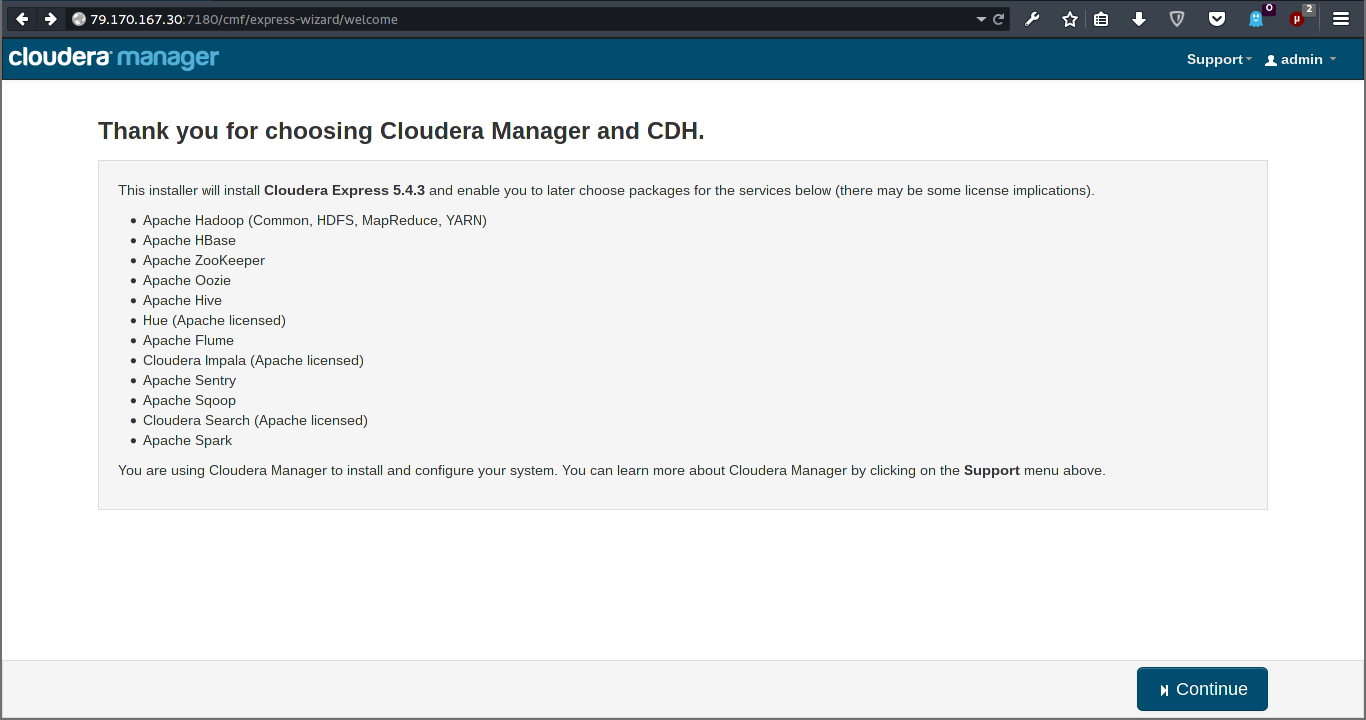
\includegraphics[width=1.0\textwidth]{image-000}
    \caption{Начальный экран установки}
    \label{img:first}
\end{figure}

\newpage

\begin{figure}[ht!]
    \center
    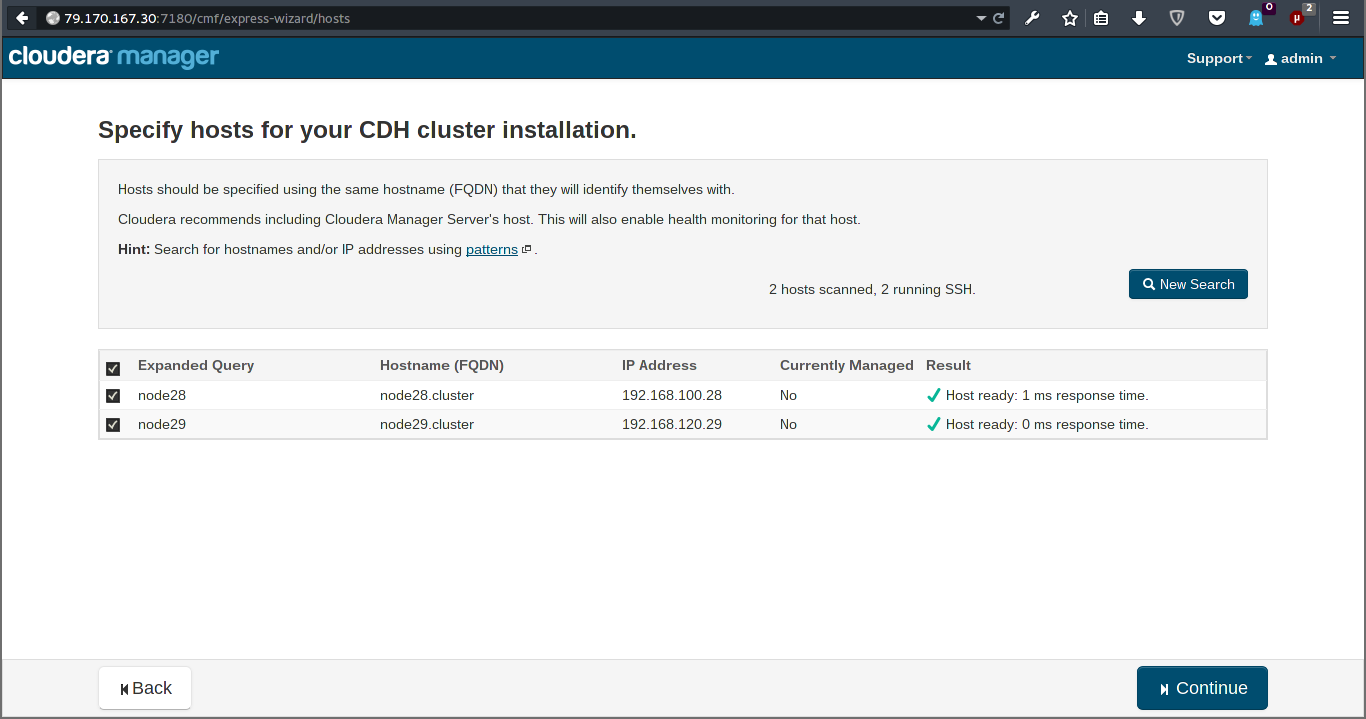
\includegraphics[width=1.0\textwidth]{image-001}
    \caption{Выбор хост-машин}
    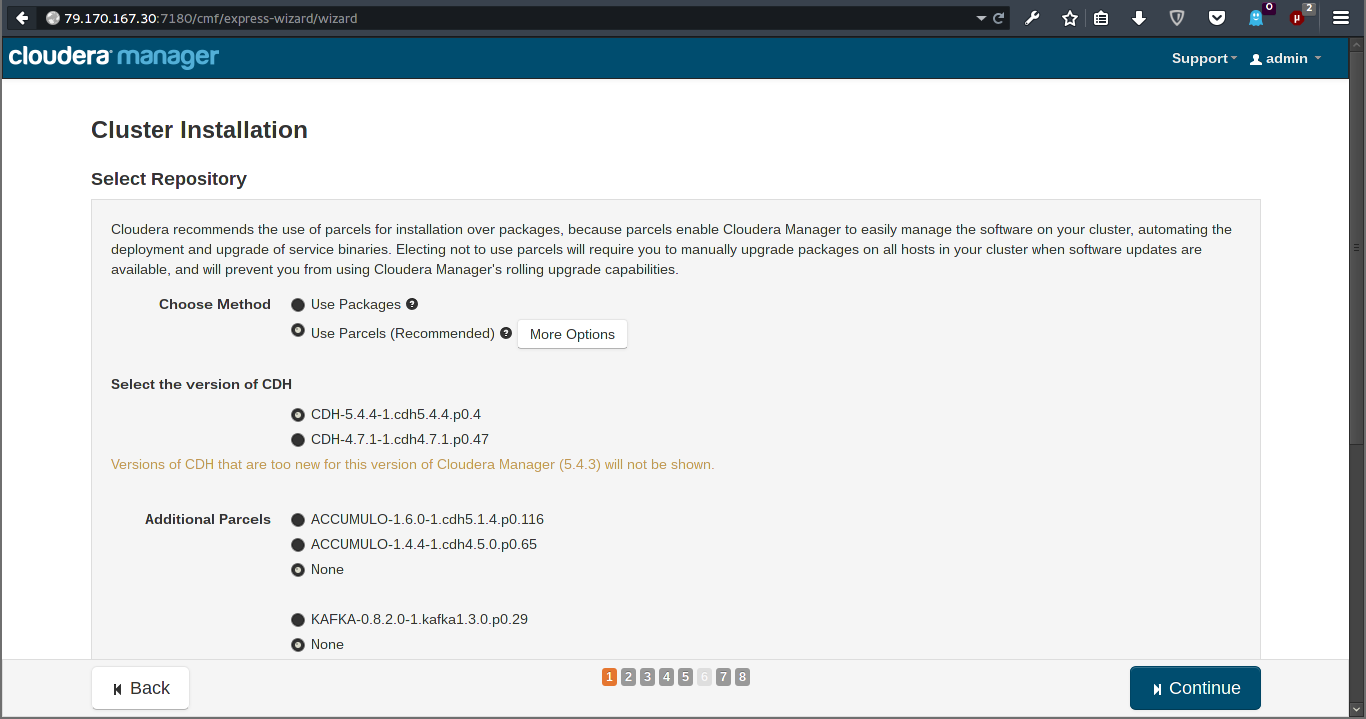
\includegraphics[width=1.0\textwidth]{image-002}
    \caption{Выбор репозитория}
\end{figure}

\newpage

\begin{figure}[ht!]
    \center
    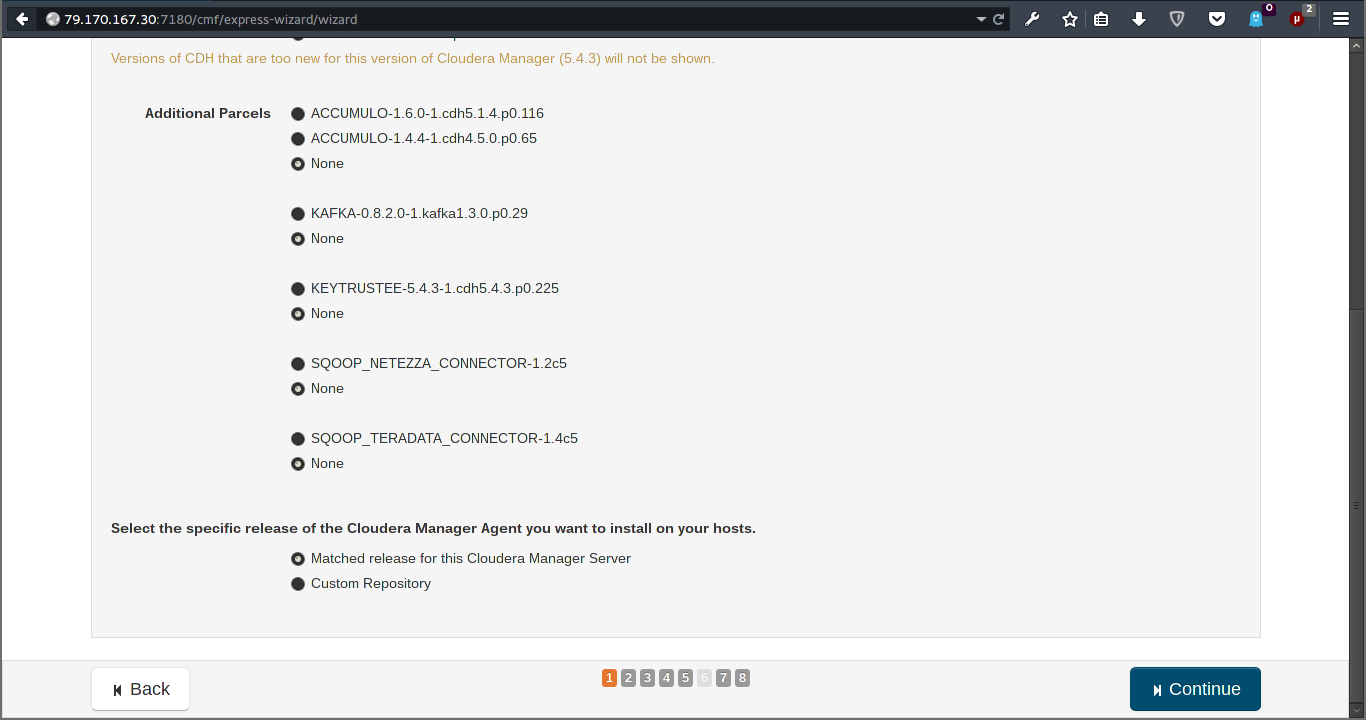
\includegraphics[width=1.0\textwidth]{image-003}
    \caption{Выбор репозитория}
    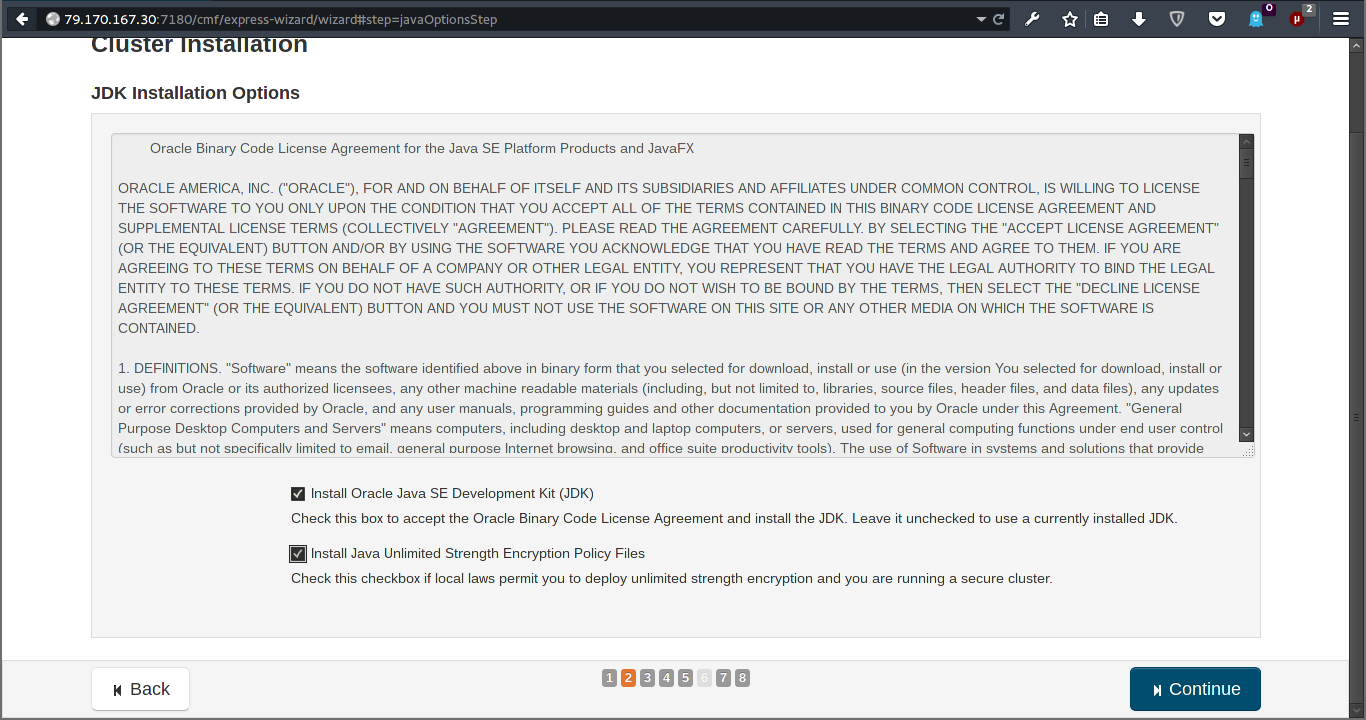
\includegraphics[width=1.0\textwidth]{image-004}
    \caption{Лицензионное соглашение}
\end{figure}

\newpage

\begin{figure}[ht!]
    \center
    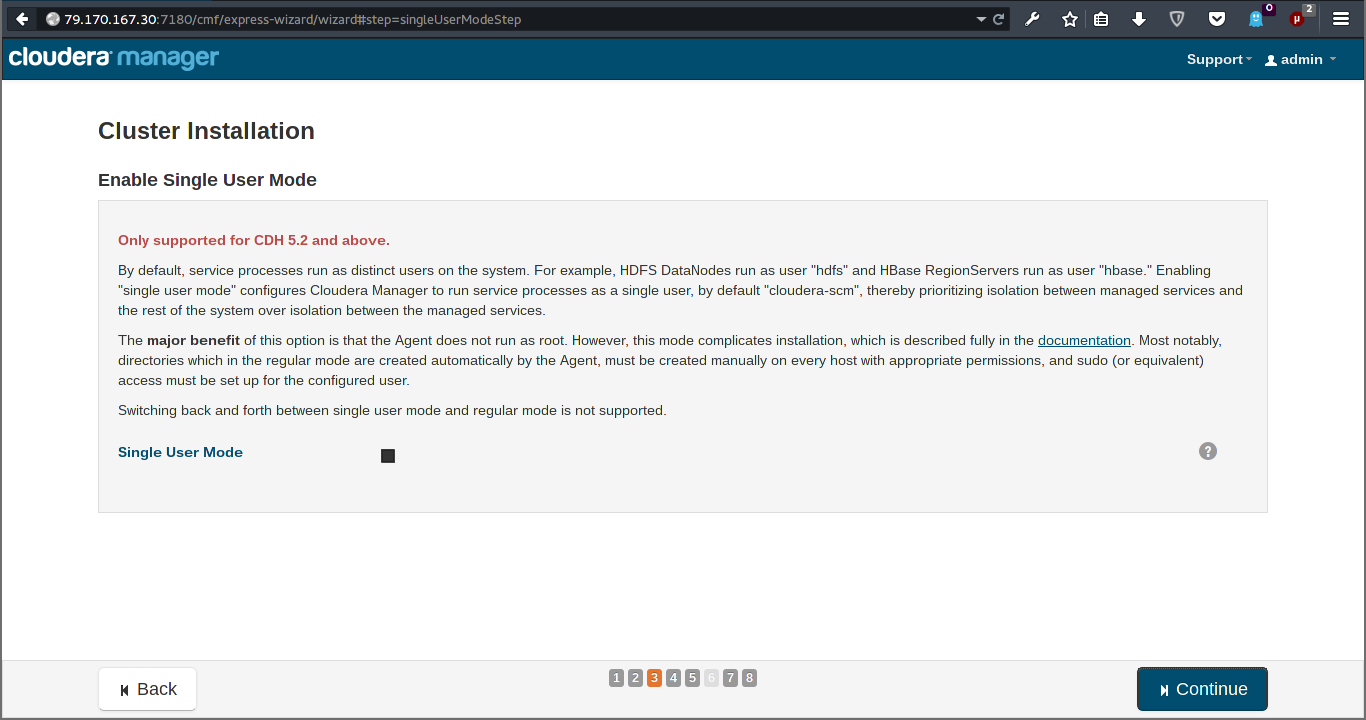
\includegraphics[width=1.0\textwidth]{image-005}
    \caption{Настройка режима установки}
    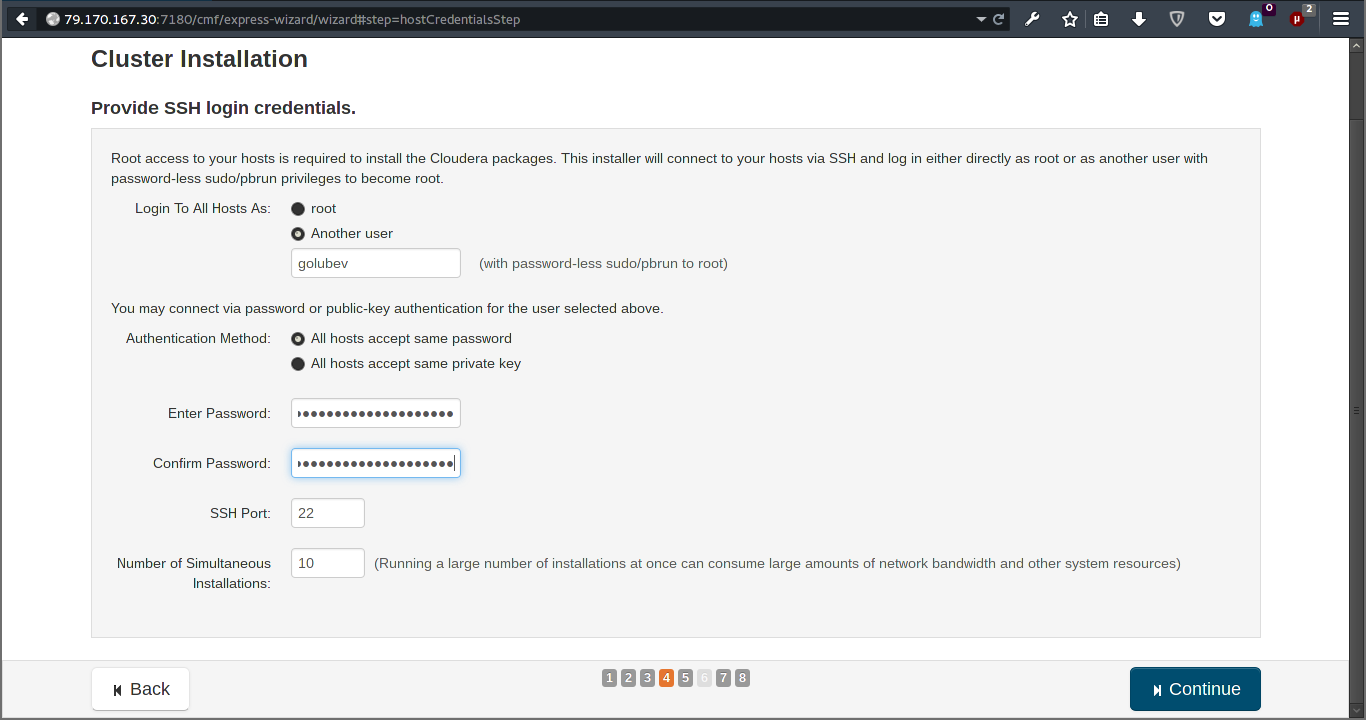
\includegraphics[width=1.0\textwidth]{image-006}
    \caption{Настройка ssh-доступа}
\end{figure}

\newpage

\begin{figure}[ht!]
    \center
    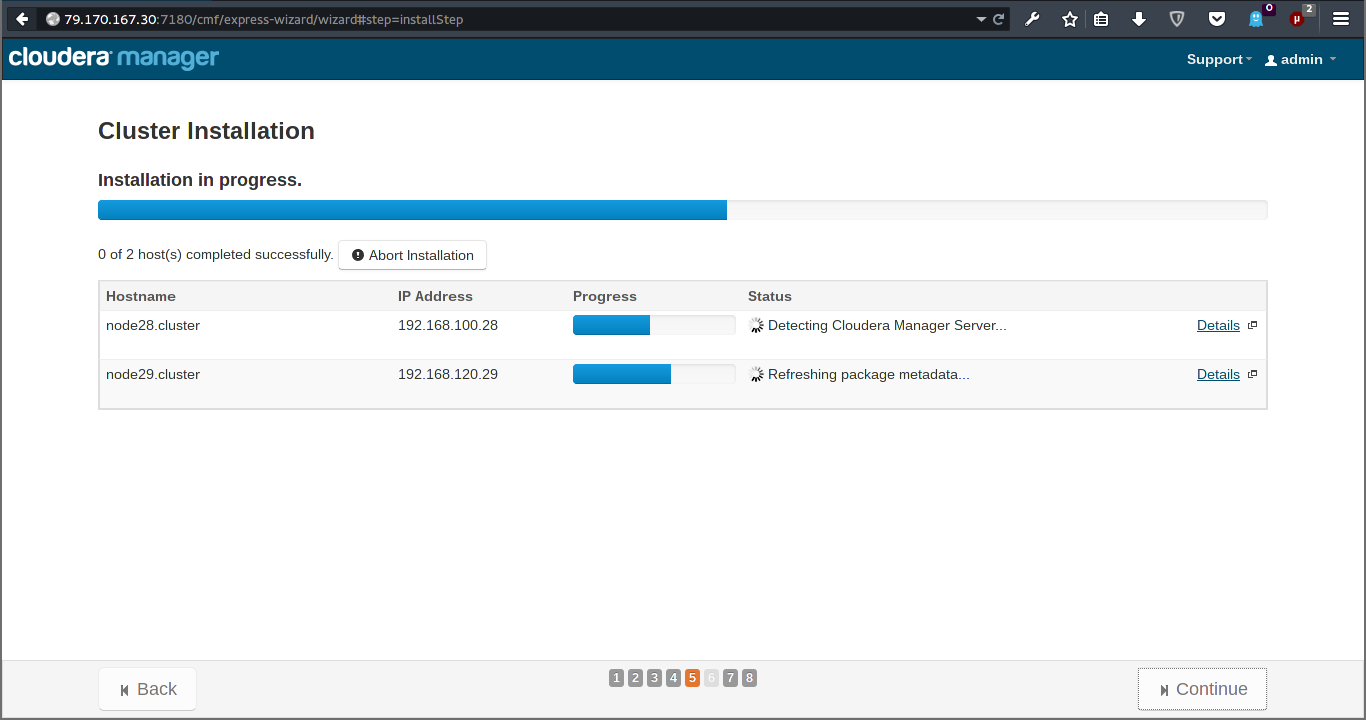
\includegraphics[width=1.0\textwidth]{image-007}
    \caption{Процесс установки}
    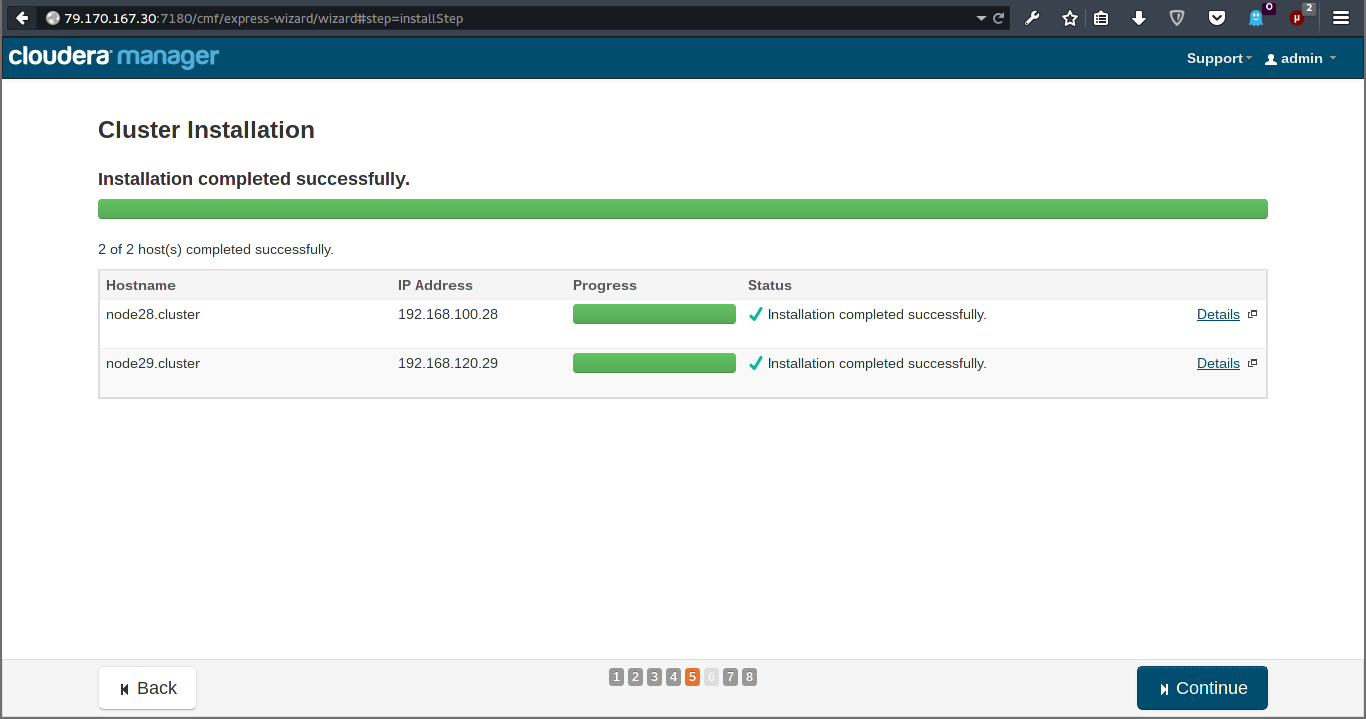
\includegraphics[width=1.0\textwidth]{image-008}
    \caption{Успешное завершение установки}
\end{figure}

В случае использования каталога \emph{/opt} как общий для всех нод необходимо произвести 
следующие действия.

Создать несколько каталогов в директории \emph{/hadoop/}
\begin{lstlisting}
$ sudo mkdir /hadoop/cloudera/csd
$ sudo /hadoop/cloudera/parcel-cache
$ sudo mkdir /hadop/cloudera/parcel-repo
$ sudo /hadoop/cloudera/parcels
\end{lstlisting}
Отредактировать файл \emph{/etc/cloudera-scm-agent/config.ini}\cite{parcels} на каждой ноде и 
перезапустить сервис
\begin{lstlisting}
$ sudo vim /etc/cloudera-scm-agent/config.ini
parcel_dir=/hadoop/cloudera/parcels
$ sudo service cloudera-scm-agent restart
\end{lstlisting}

Далее переходим на главную страницу Cloudera Manager во вкладку \\
Hosts->Configuration, где устанавливаем следующие параметры
\begin{itemize}
    \item Parcel Directory
    \item Local Parcel Repository Path
\end{itemize}

\begin{figure}[ht!]
    \center
    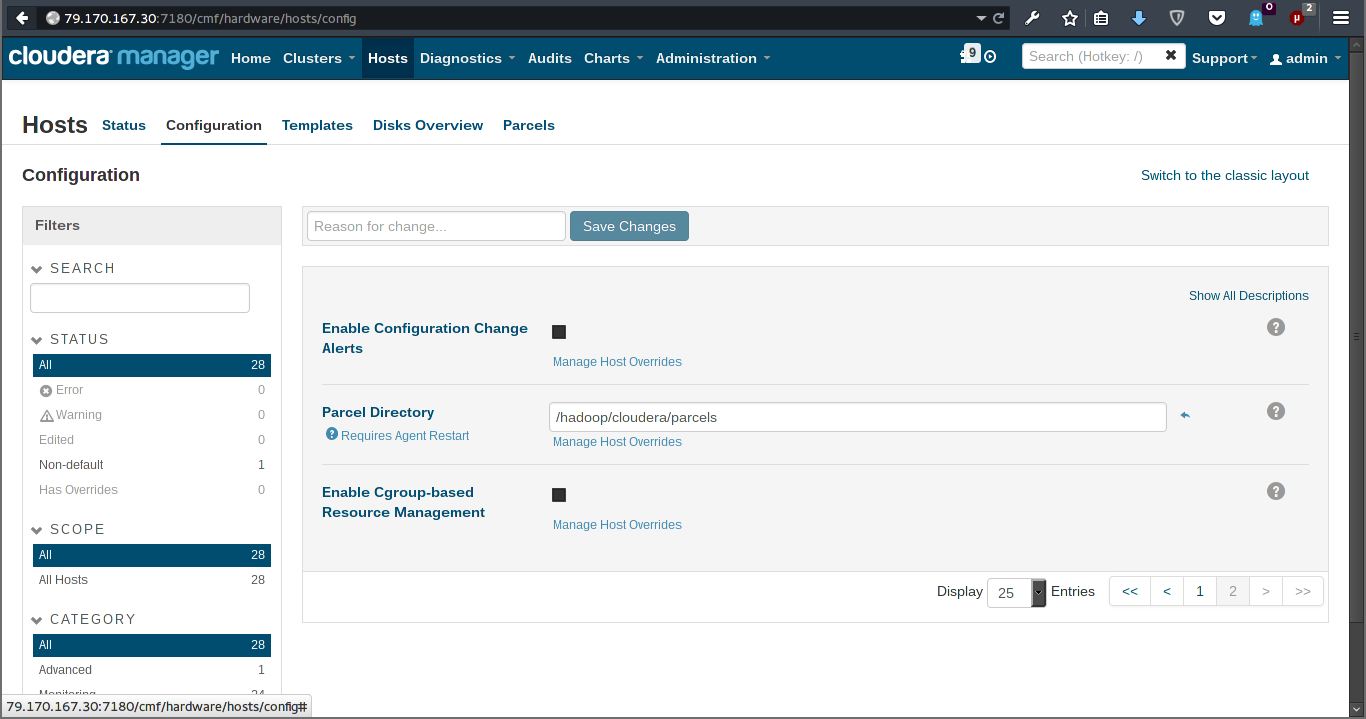
\includegraphics[width=0.8\textwidth]{image-009}
    \caption{Конфигурация параметров}
    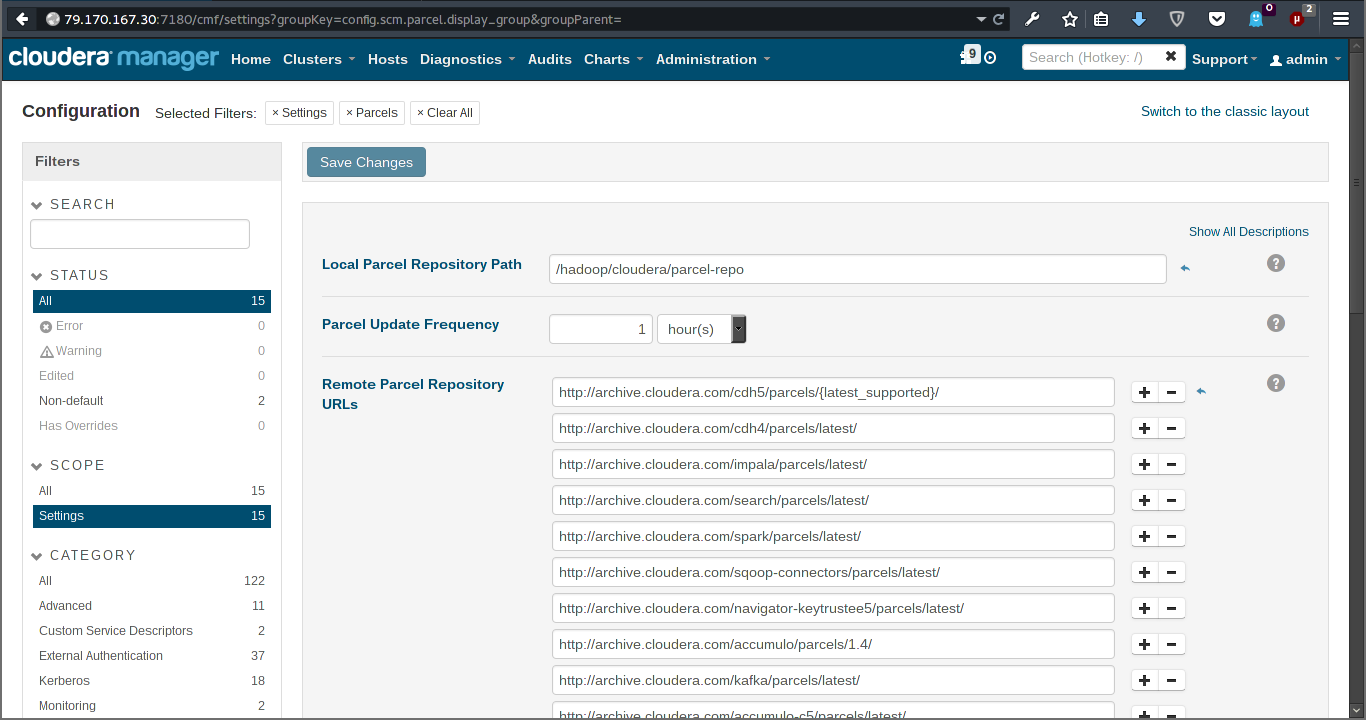
\includegraphics[width=0.8\textwidth]{image-010}
    \caption{Конфигурация параметров}
\end{figure}
Переходим на главную страницу, выбираем \emph{Add Service} и продолжаем установку.

\newpage

\begin{figure}[ht!]
    \center
    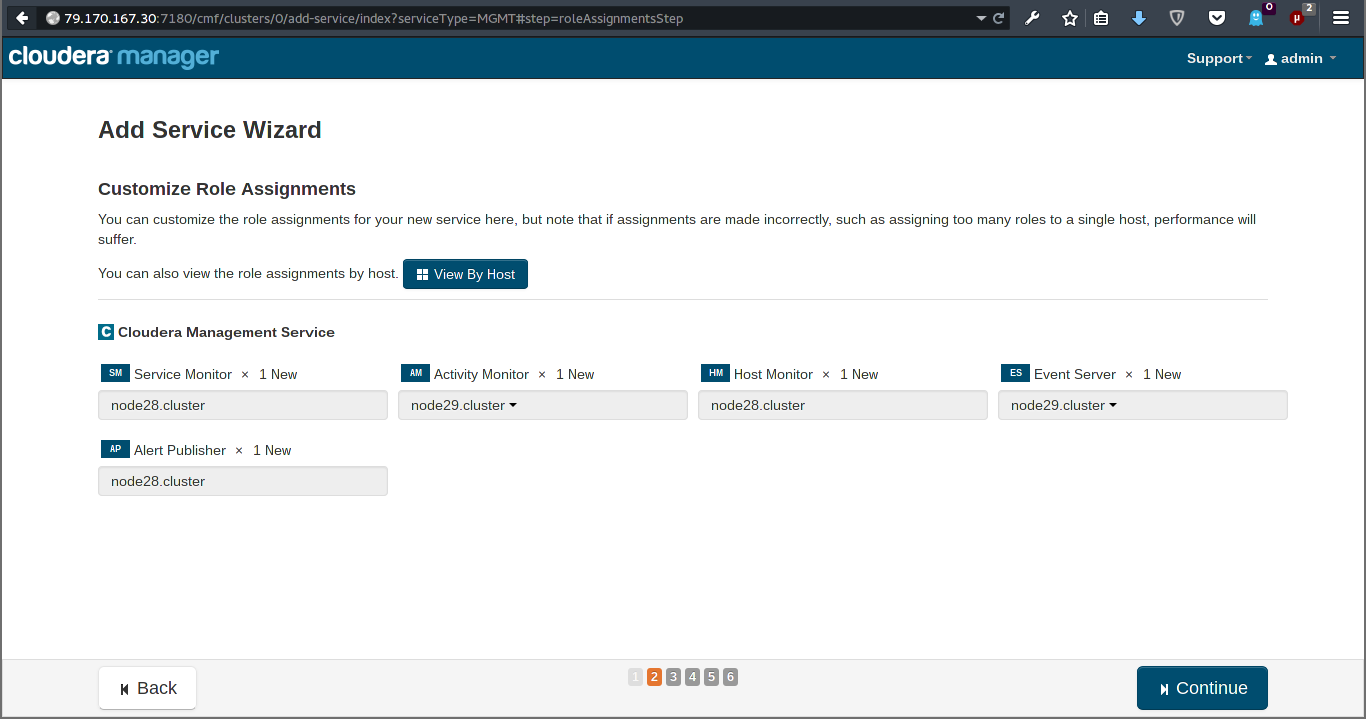
\includegraphics[width=1.0\textwidth]{image-011}
    \caption{Установка Cloudera Manager Service}
    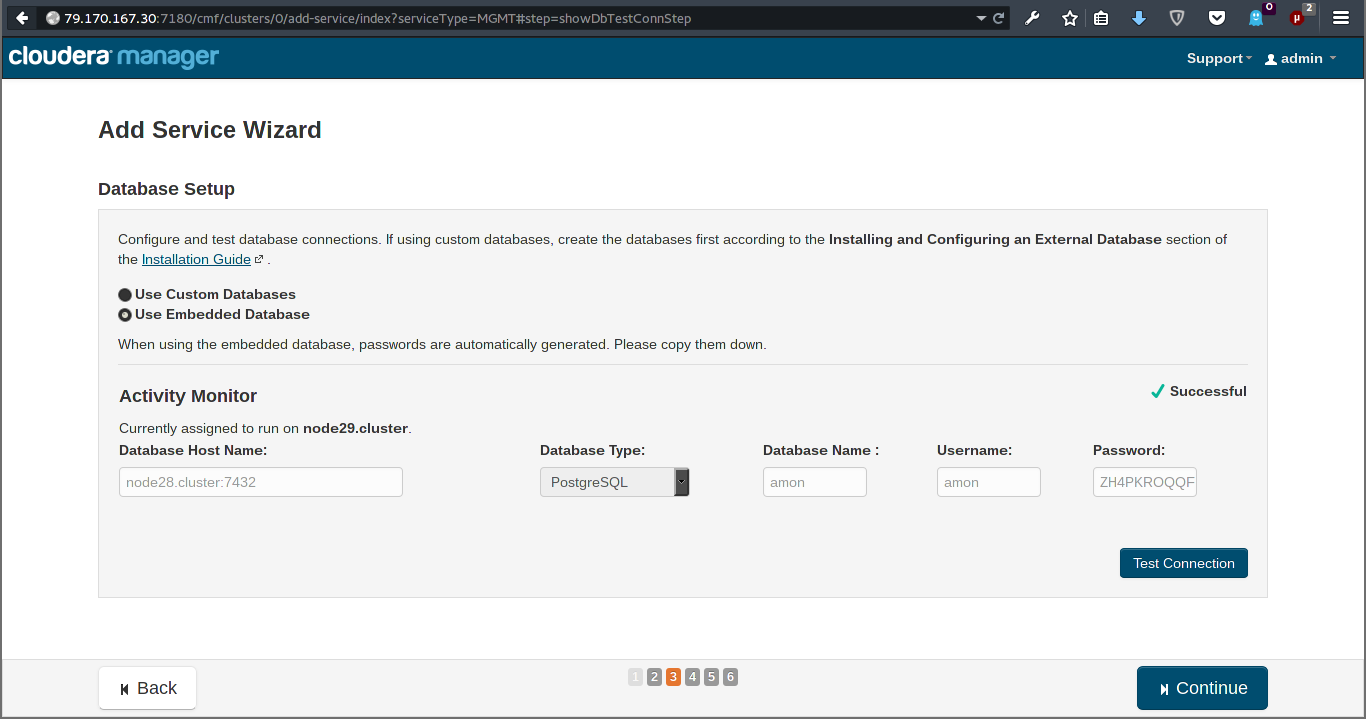
\includegraphics[width=1.0\textwidth]{image-012}
    \caption{Подключение к БД}
\end{figure}

\newpage

\begin{figure}[ht!]
    \center
    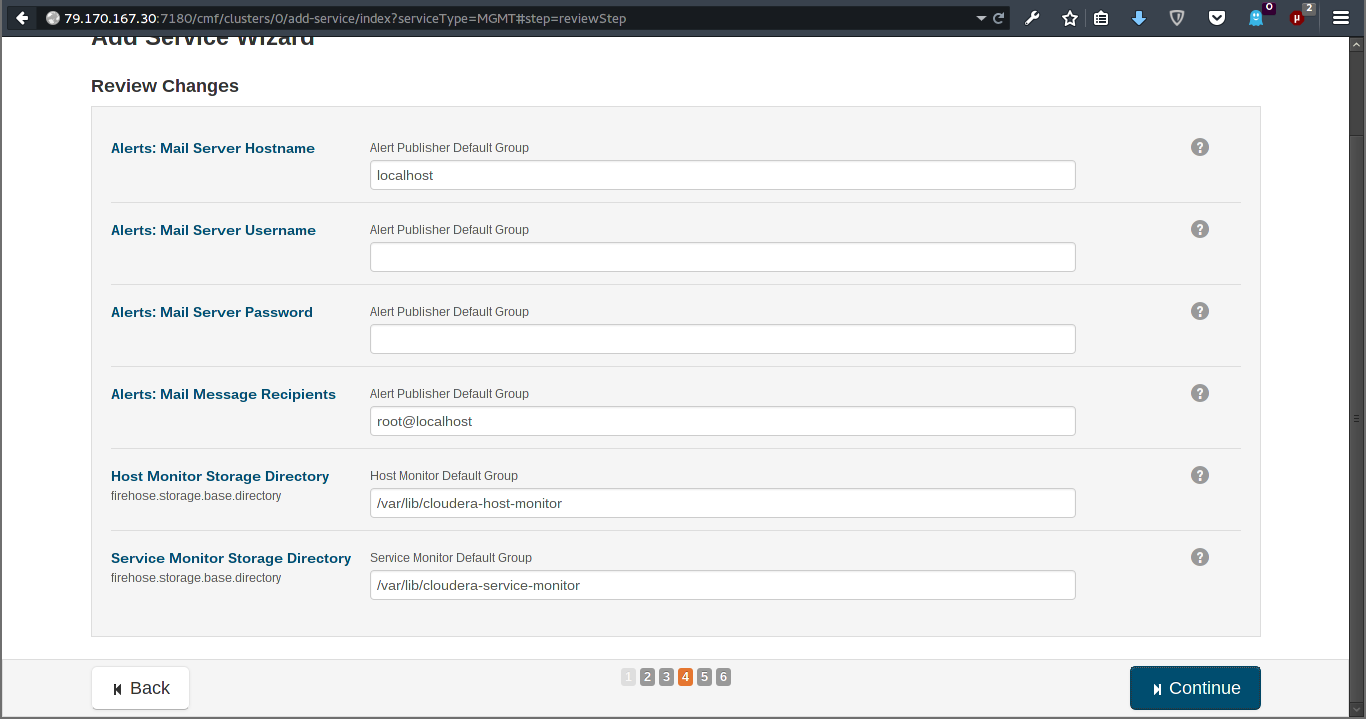
\includegraphics[width=1.0\textwidth]{image-013}
    \caption{Конфигурация сервиса}
    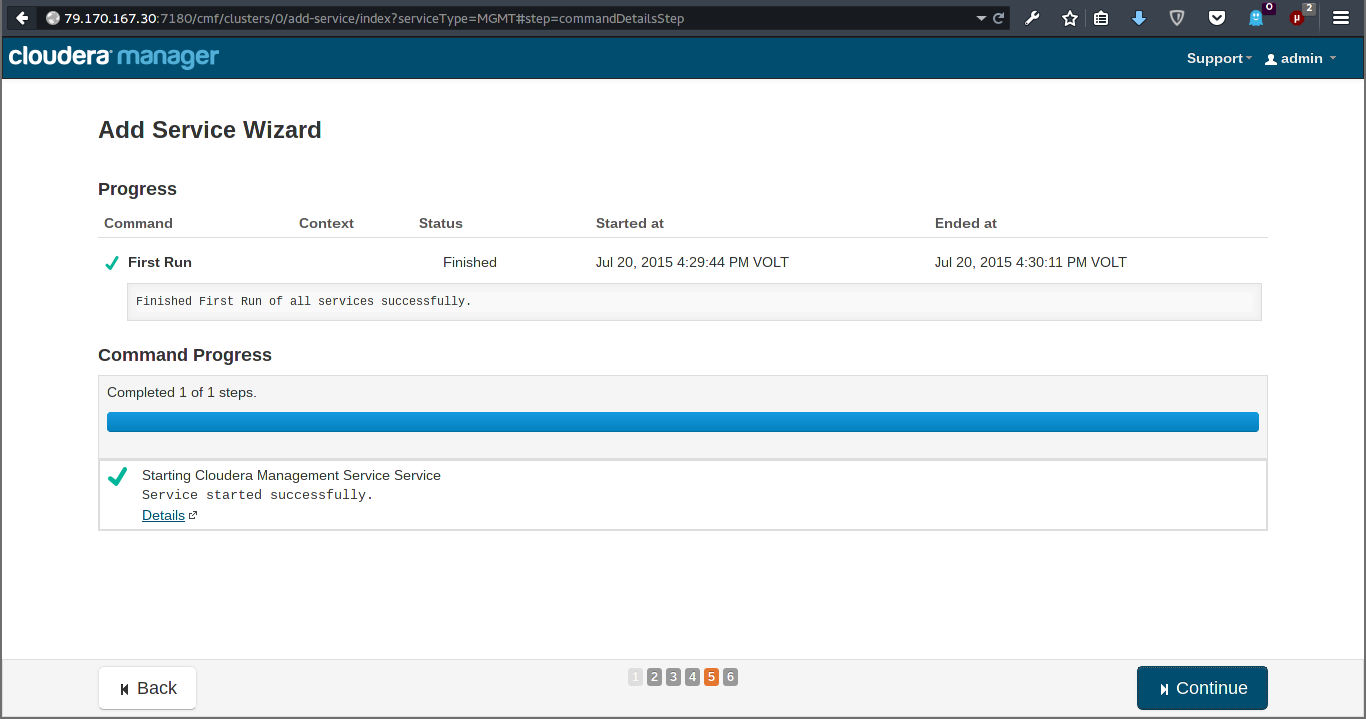
\includegraphics[width=1.0\textwidth]{image-014}
    \caption{Процесс установки}
\end{figure}

Если вы изменили параметры \emph{Parcel Directory}, то выйдете на главную страницу страницу и 
создайте кластер с параметрами из шагов ранее. Установка основных пакетов Cloudera Manager 
может длиться значительное время.

\newpage

\begin{figure}[ht!]
    \center
    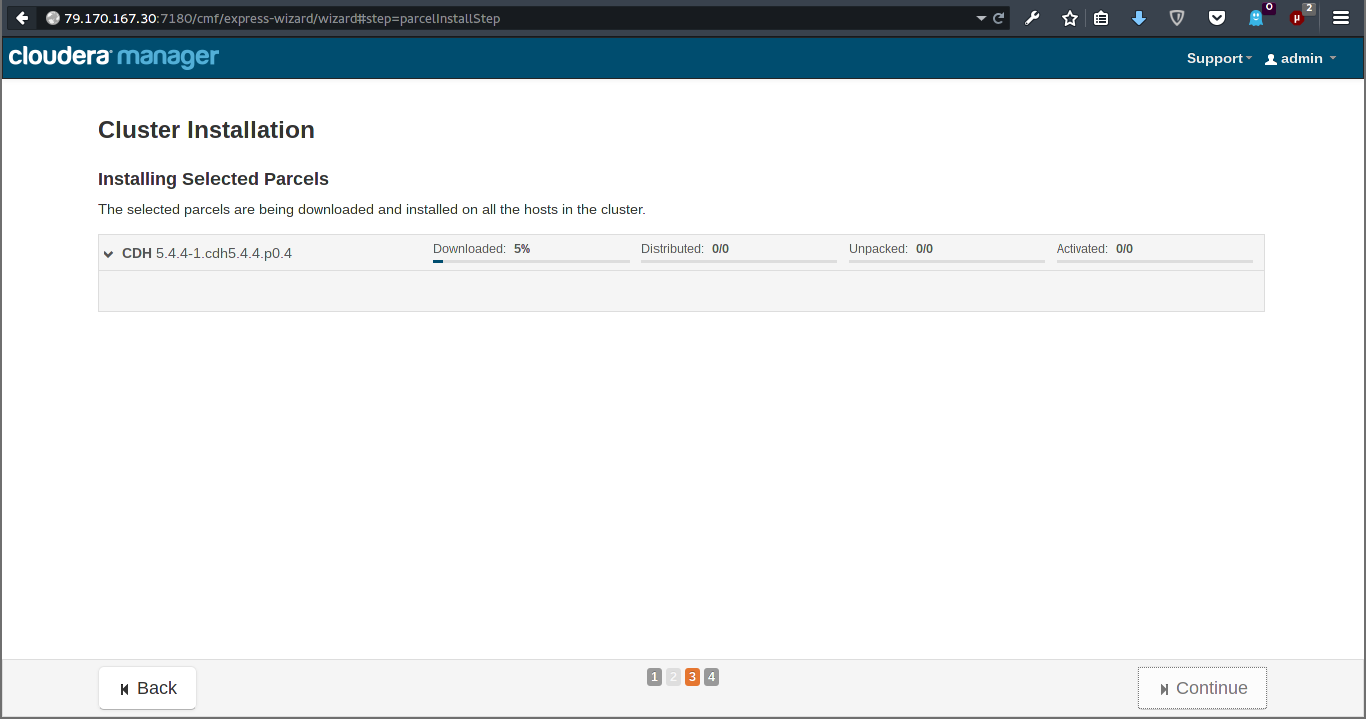
\includegraphics[width=1.0\textwidth]{image-020}
    \caption{Установка CDH}
    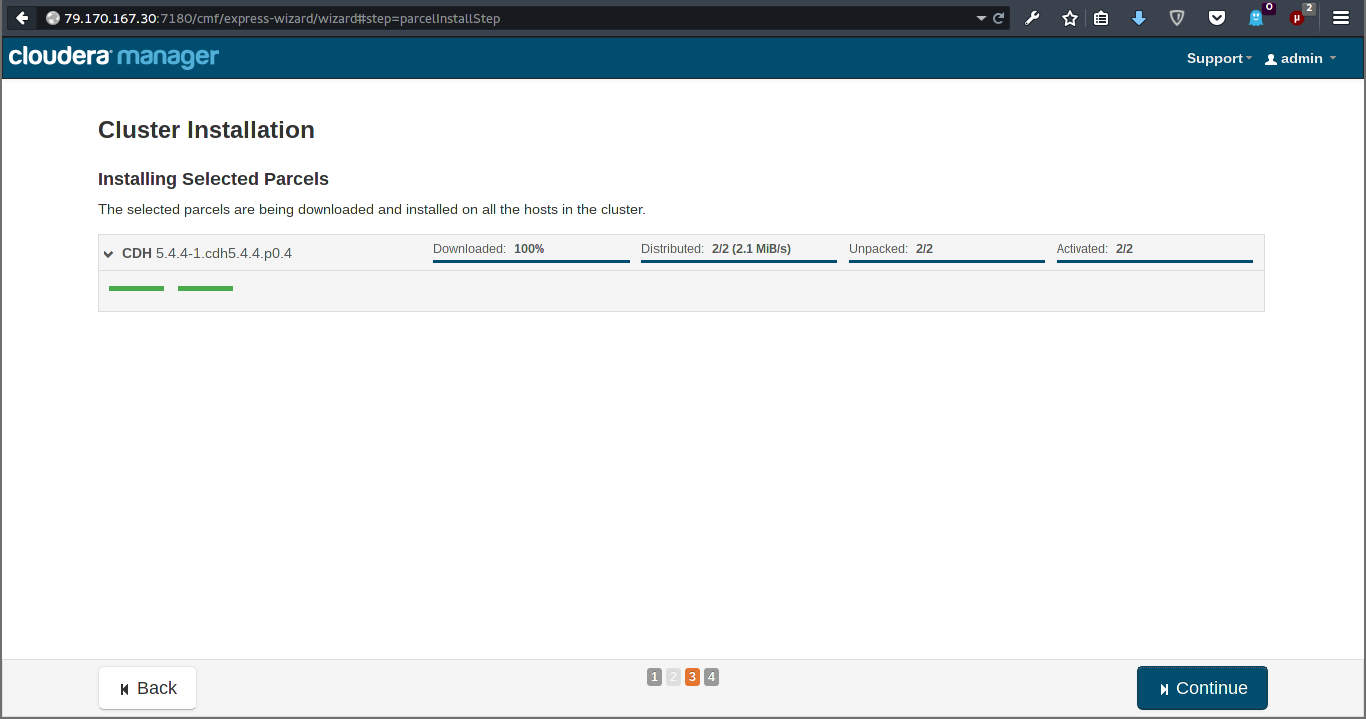
\includegraphics[width=1.0\textwidth]{image-021}
    \caption{Успешное завершение установки}
\end{figure}

\newpage

\begin{figure}[ht!]
    \center
    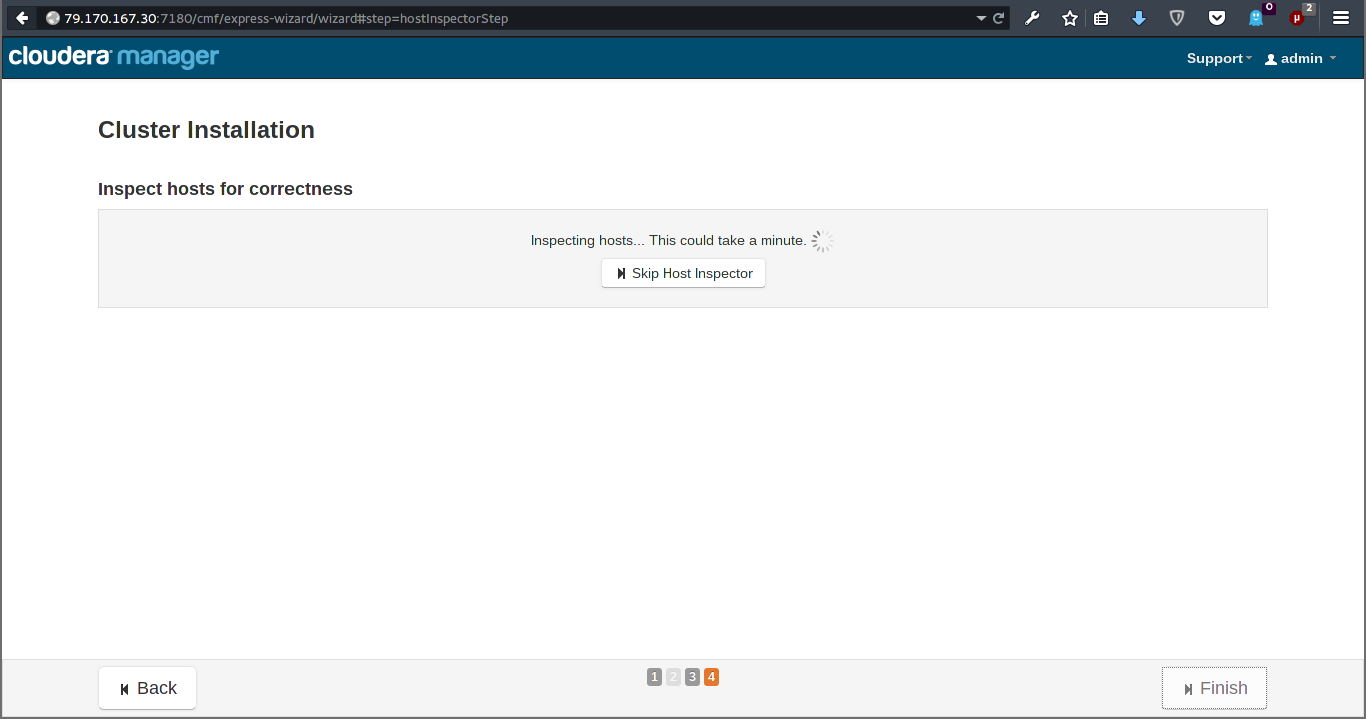
\includegraphics[width=1.0\textwidth]{image-022}
    \caption{Проверка хост-машин}
    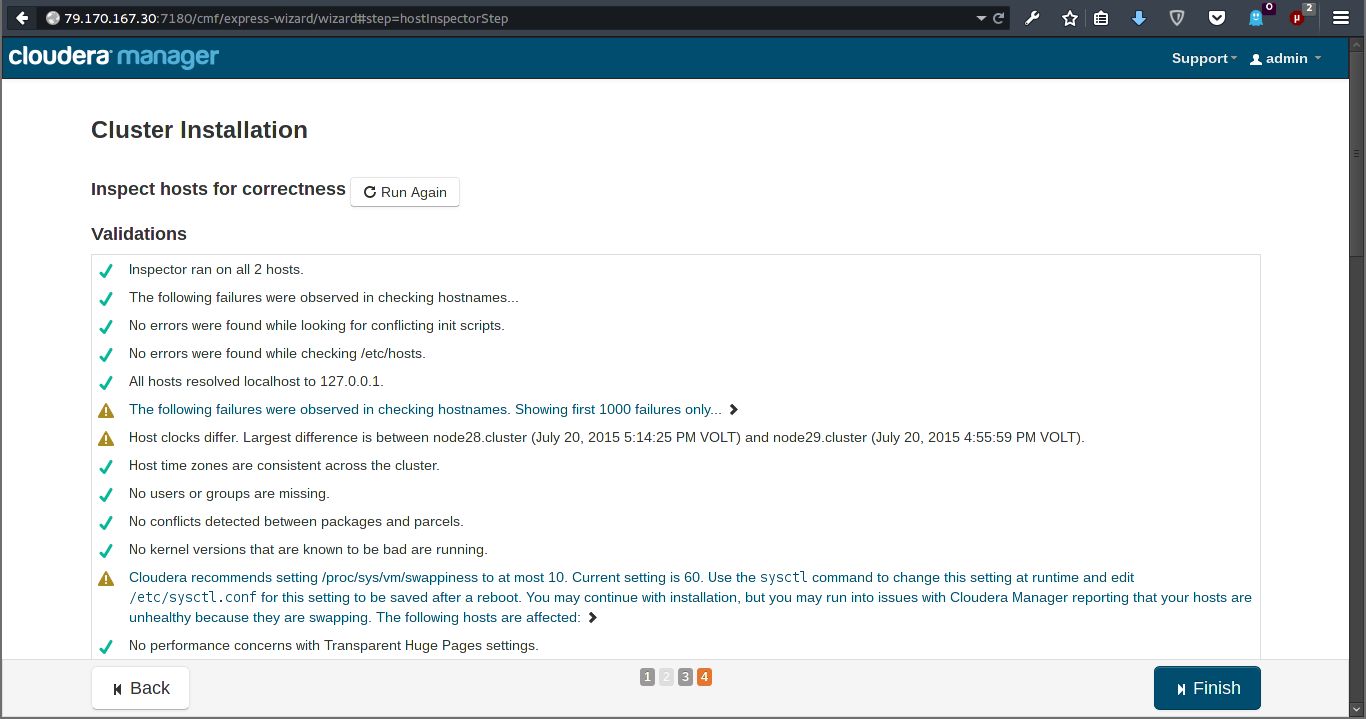
\includegraphics[width=1.0\textwidth]{image-023}
    \caption{Результат проверки хост-машин}
\end{figure}

\newpage

\begin{figure}[ht!]
    \center
    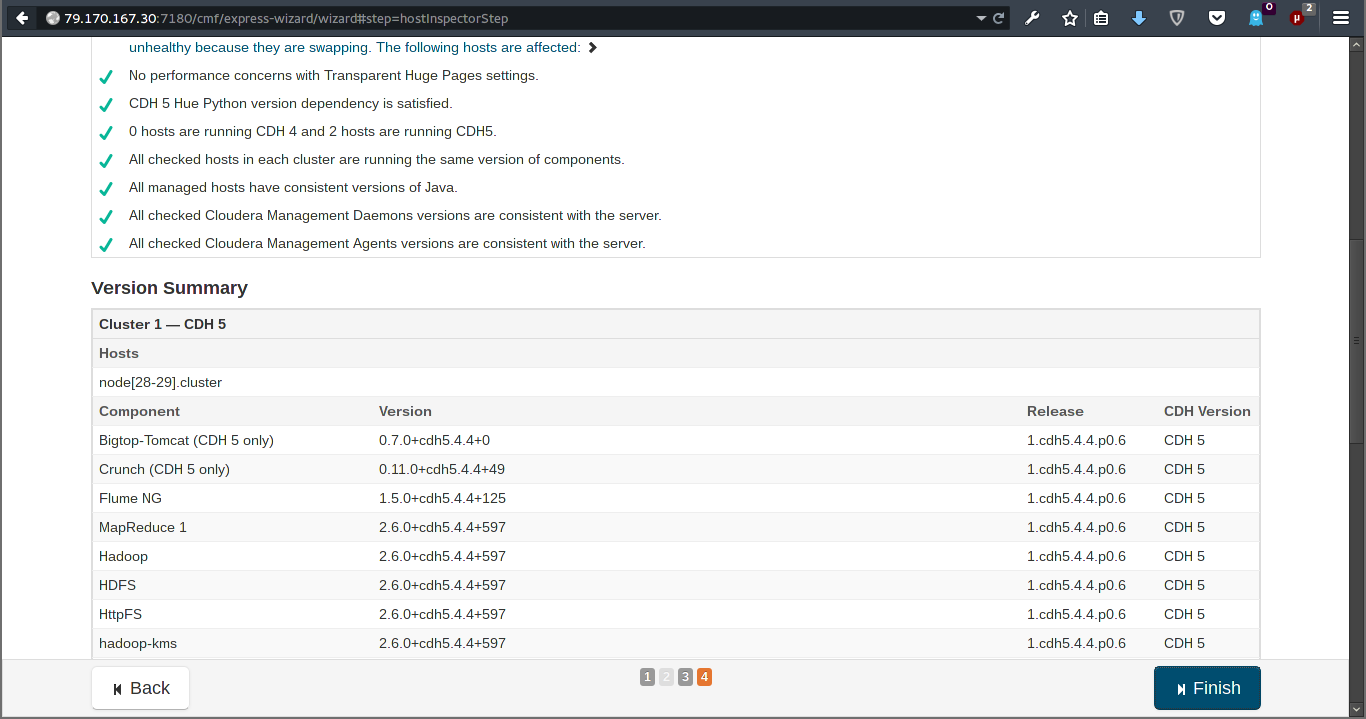
\includegraphics[width=1.0\textwidth]{image-024}
    \caption{Результат проверки хост-машин}
    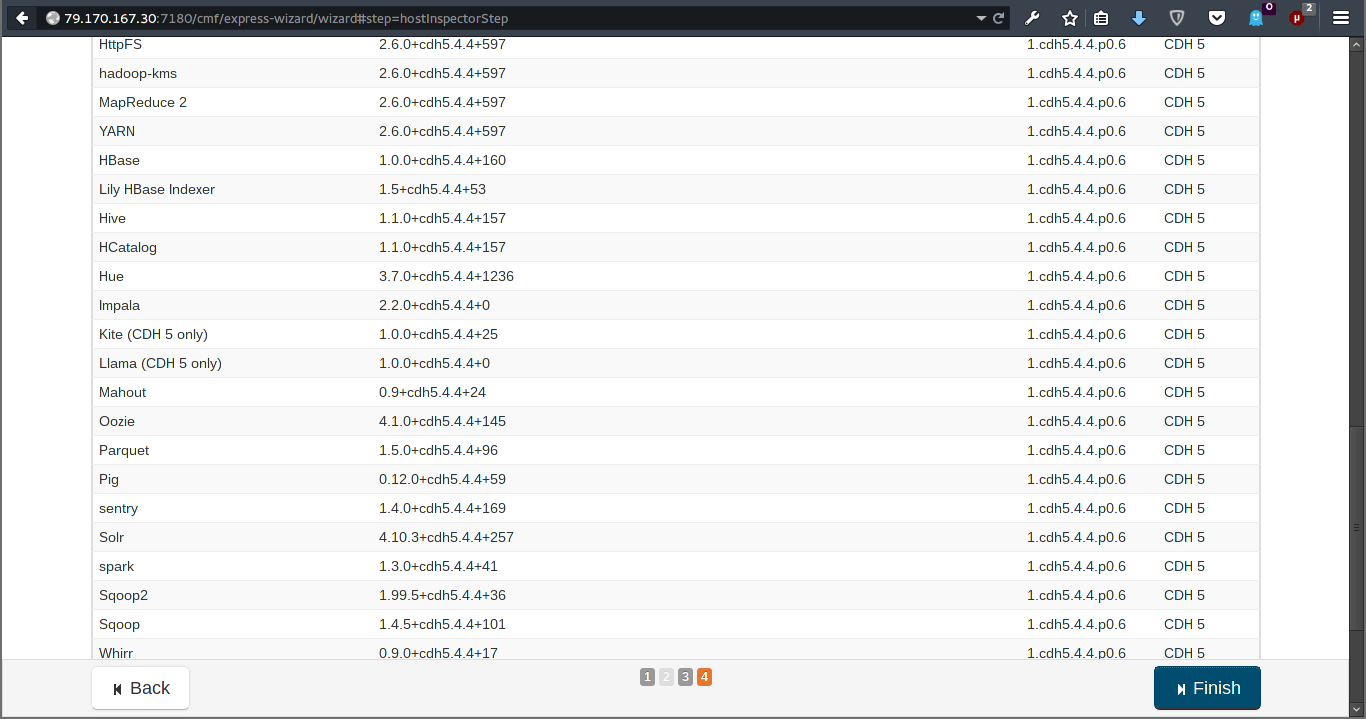
\includegraphics[width=1.0\textwidth]{image-025}
    \caption{Результат проверки хост-машин}
\end{figure}

\newpage

\begin{figure}[ht!]
    \center
    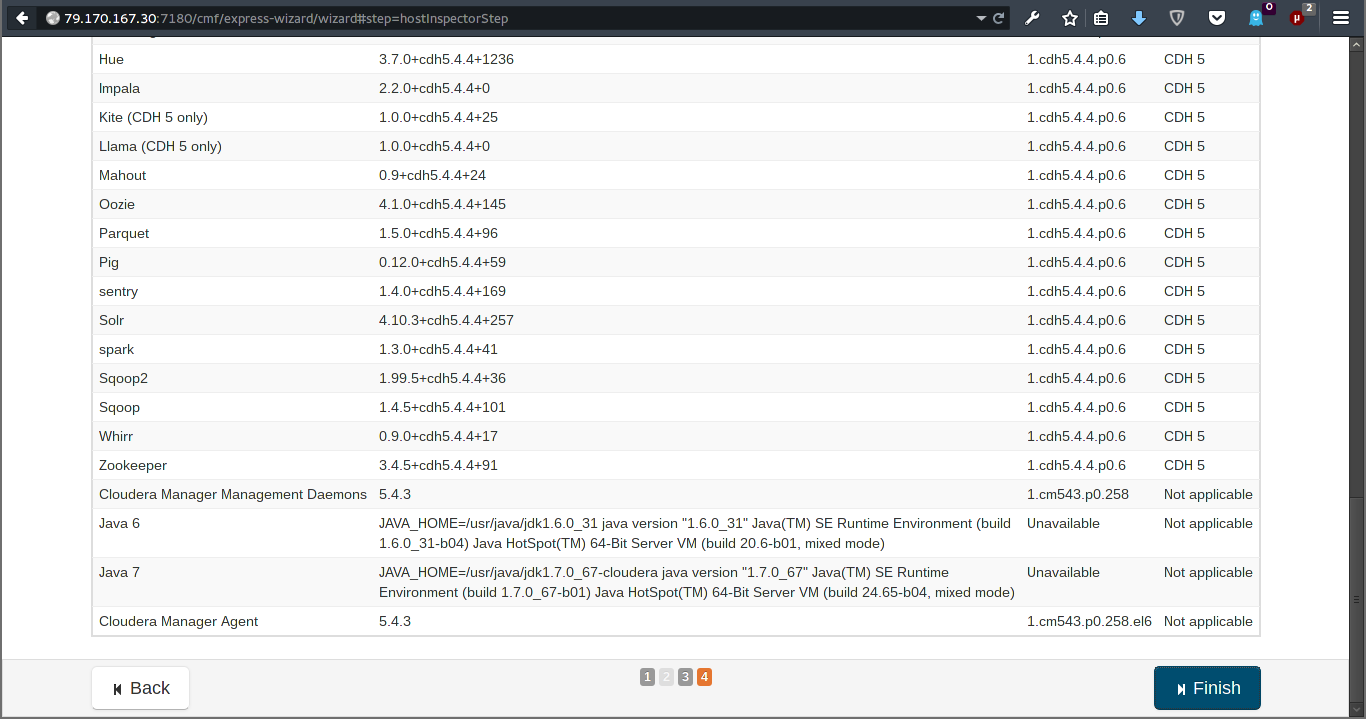
\includegraphics[width=1.0\textwidth]{image-026}
    \caption{Результат проверки хост-машин}
    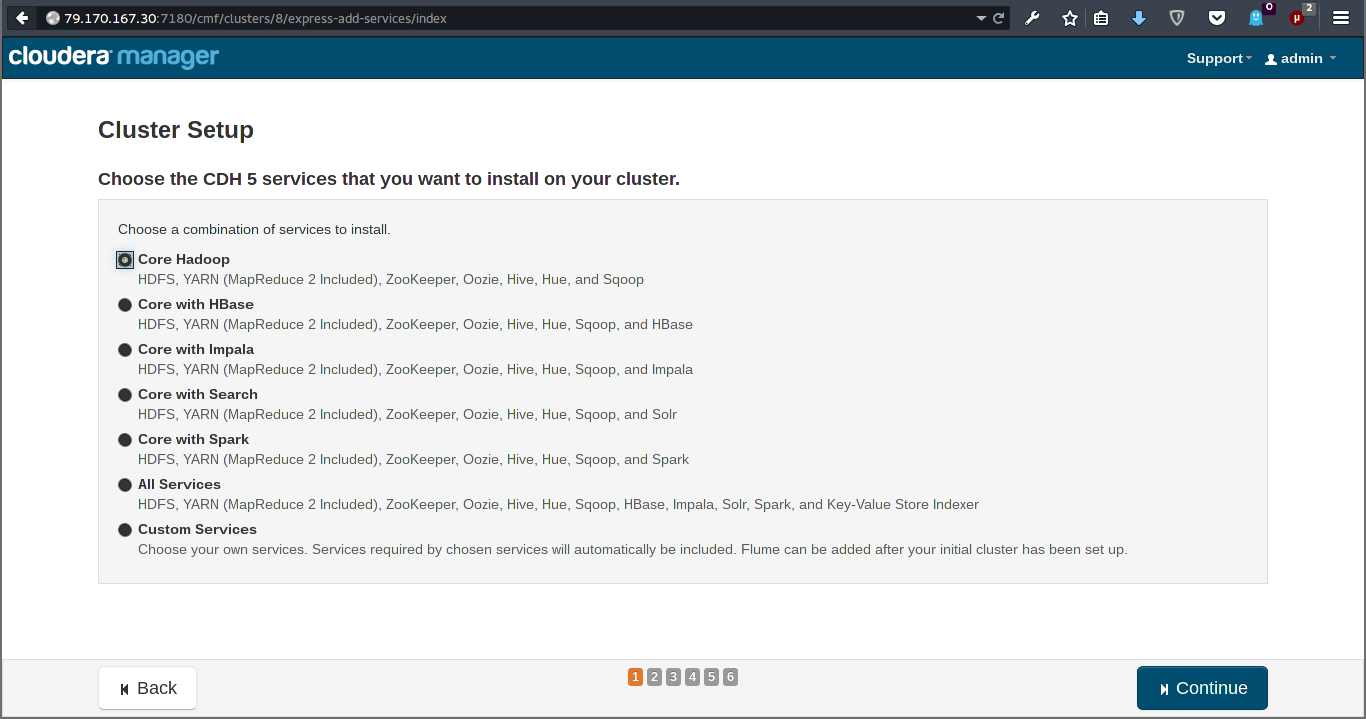
\includegraphics[width=1.0\textwidth]{image-027}
    \caption{Выбор устанавливаемых компонентов}
\end{figure}

\newpage

\begin{figure}[ht!]
    \center
    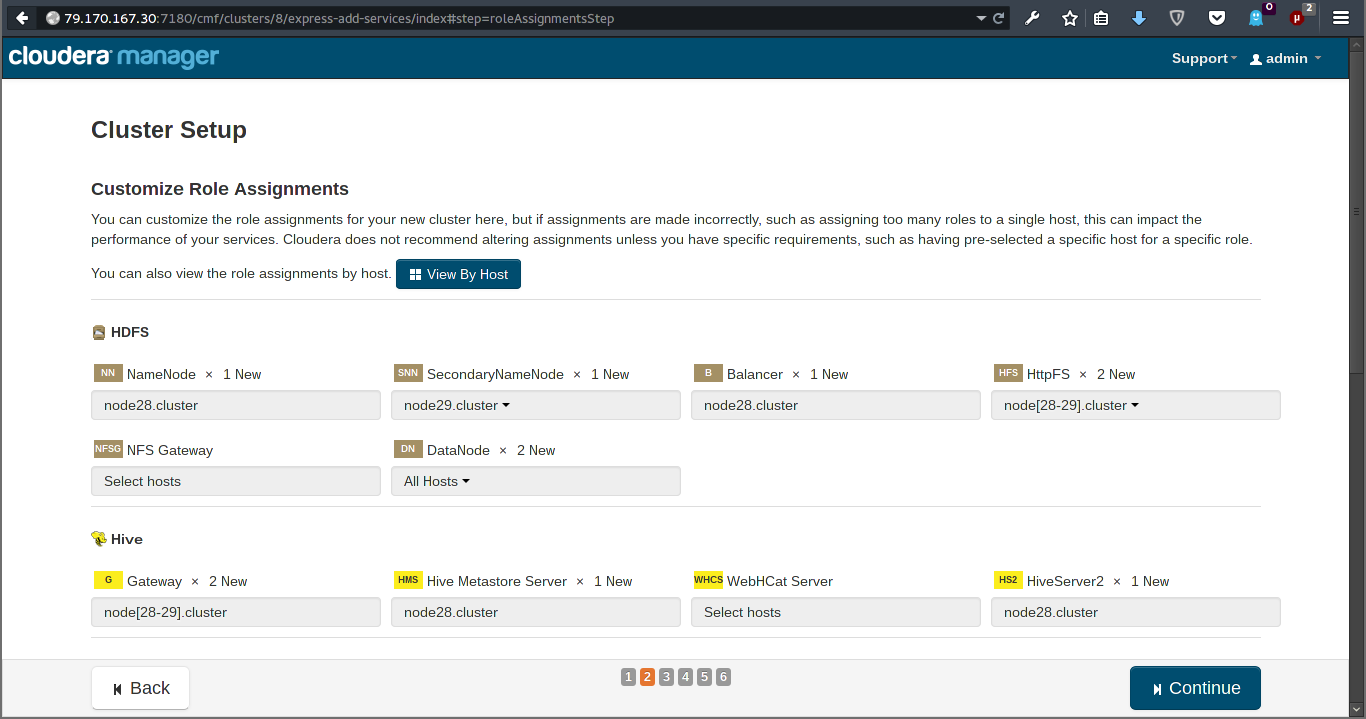
\includegraphics[width=1.0\textwidth]{image-028}
    \caption{Конфигурация ролей хост-машин}
    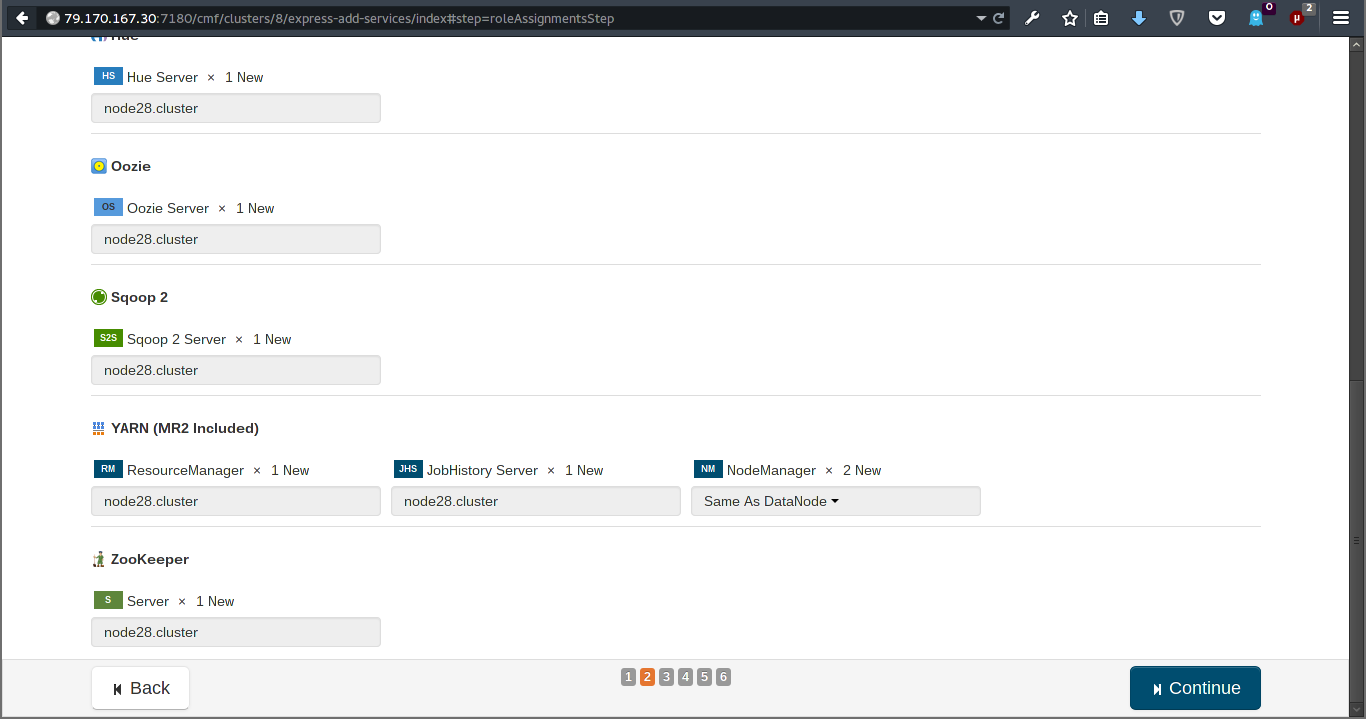
\includegraphics[width=1.0\textwidth]{image-029}
    \caption{Конфигурация ролей хост-машин}
\end{figure}

\newpage

\begin{figure}[ht!]
    \center
    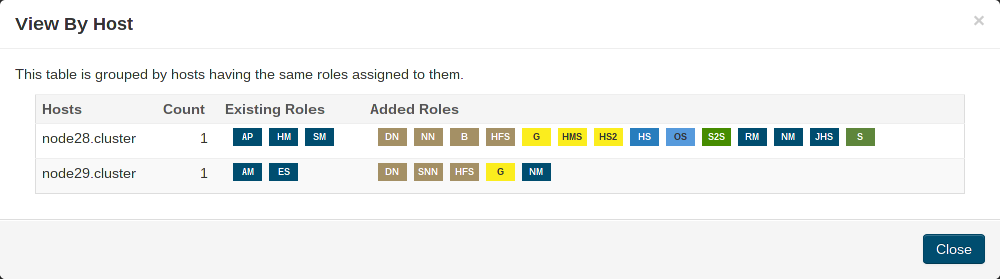
\includegraphics[width=1.0\textwidth]{image-030}
    \caption{Распределение ролей хост-машин}
    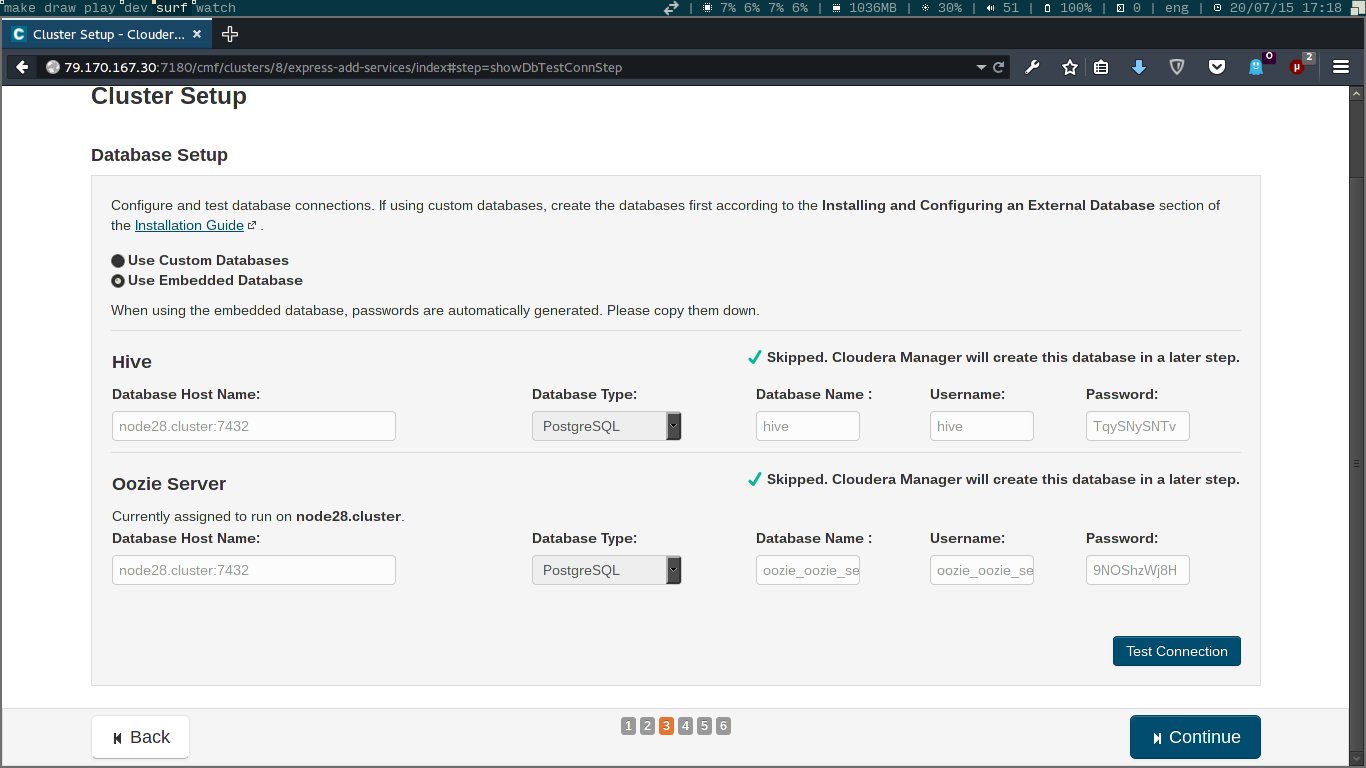
\includegraphics[width=1.0\textwidth]{image-031}
    \caption{Подключение БД}
    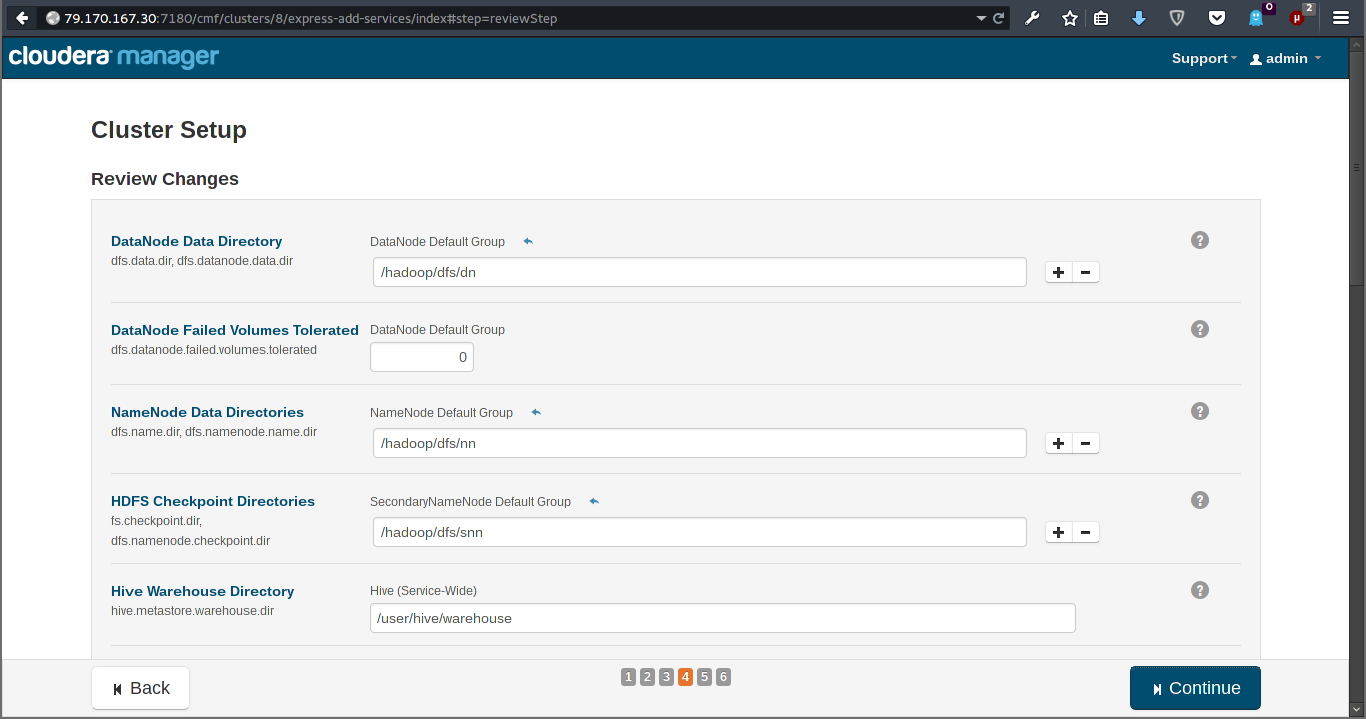
\includegraphics[width=1.0\textwidth]{image-032}
    \caption{Конфигурация параметров}
\end{figure}

\newpage

\begin{figure}[ht!]
    \center
    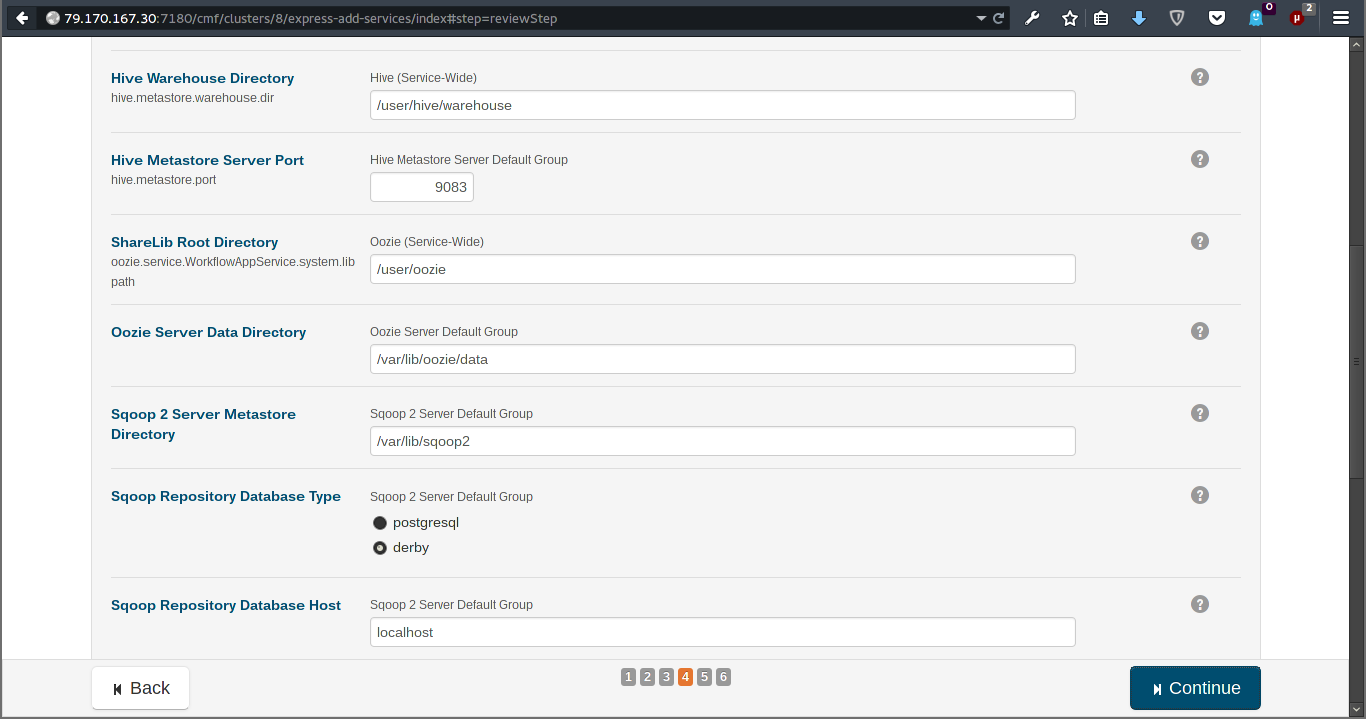
\includegraphics[width=1.0\textwidth]{image-033}
    \caption{Конфигурация параметров}
    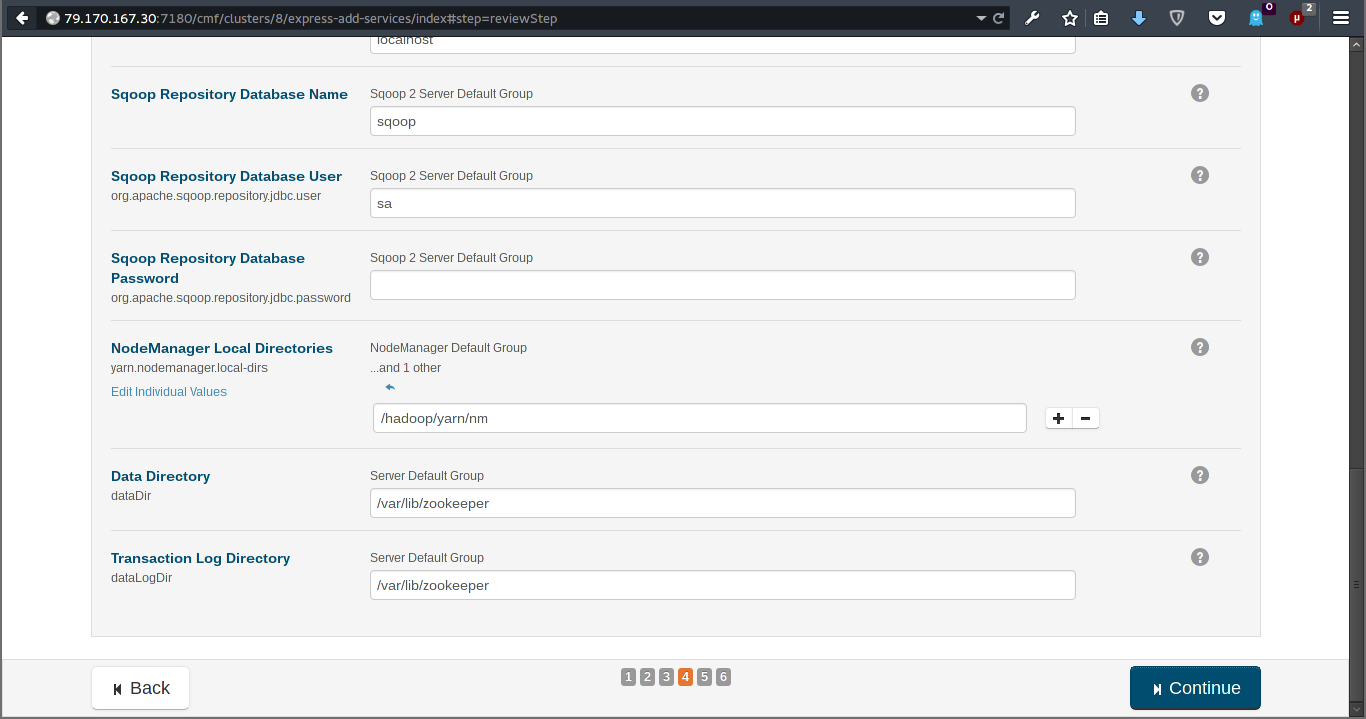
\includegraphics[width=1.0\textwidth]{image-034}
    \caption{Конфигурация параметров}
\end{figure}

\newpage

\begin{figure}[ht!]
    \center
    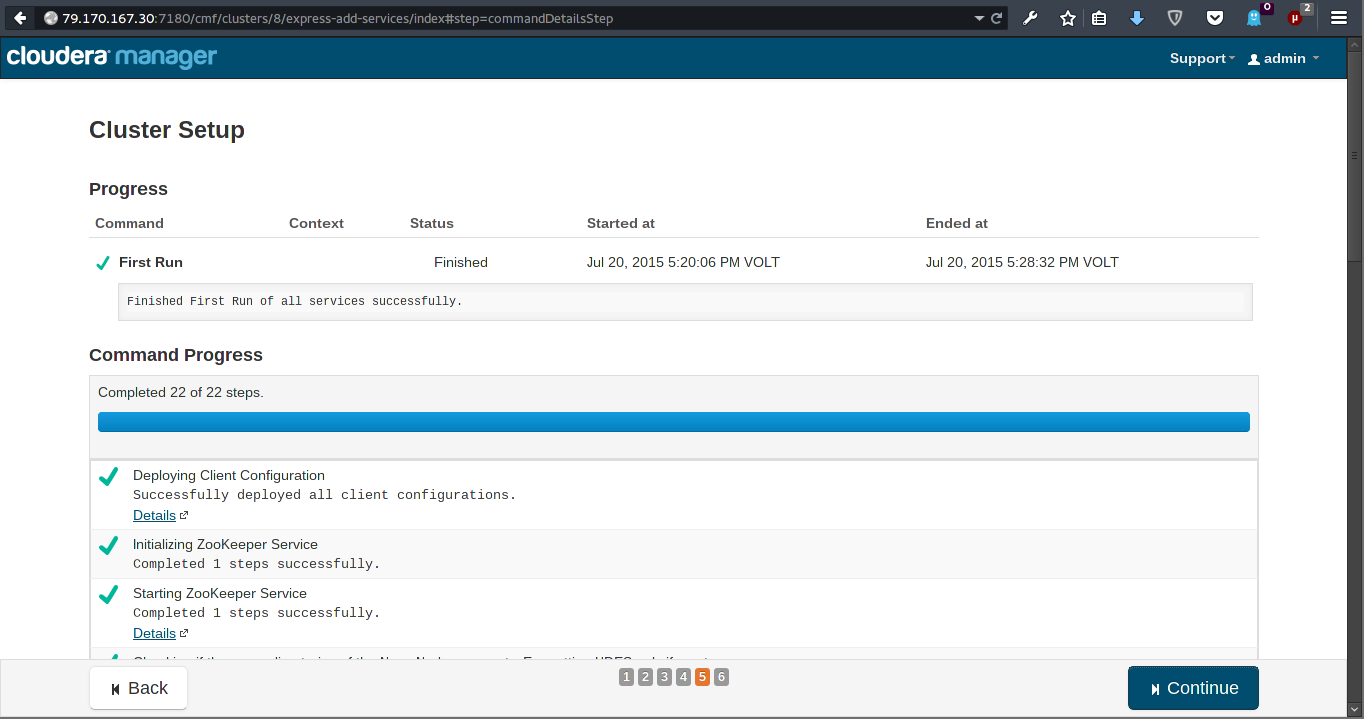
\includegraphics[width=1.0\textwidth]{image-035}
    \caption{Процесс установки}
    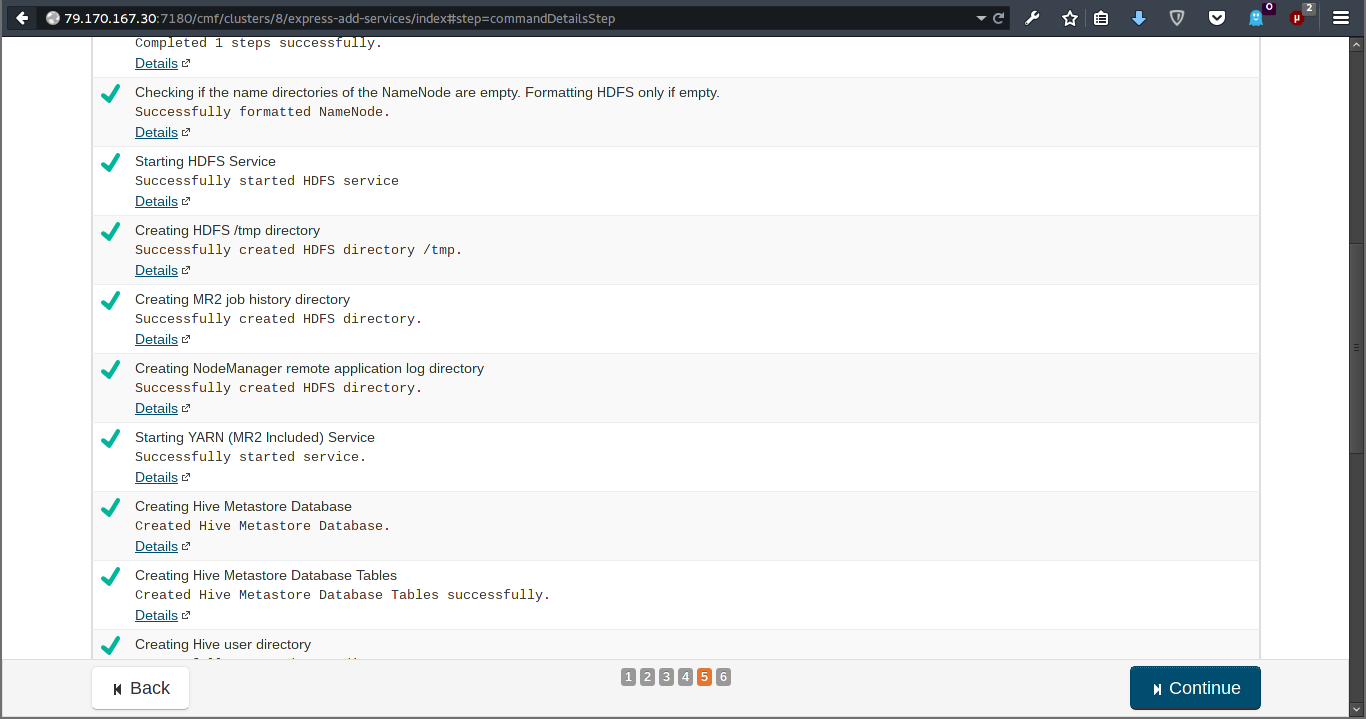
\includegraphics[width=1.0\textwidth]{image-036}
    \caption{Успешная установка компонентов}
\end{figure}

\newpage

\begin{figure}[ht!]
    \center
    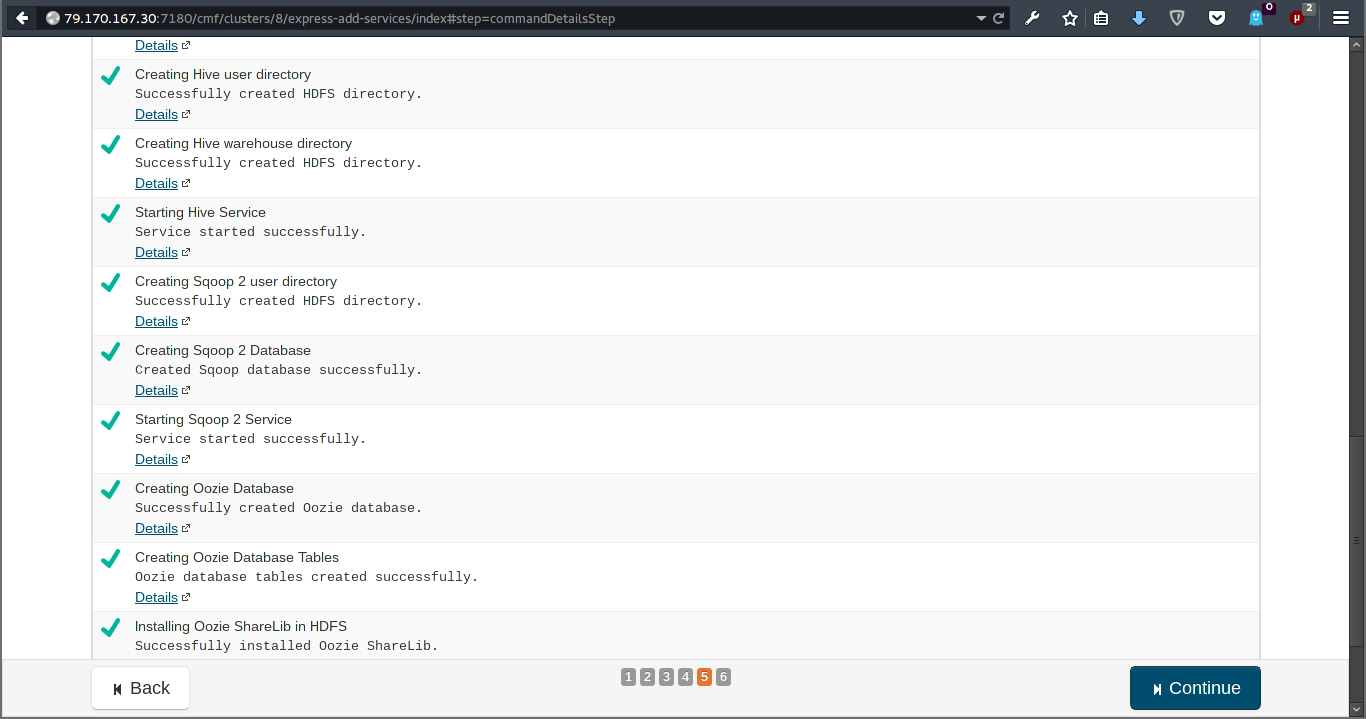
\includegraphics[width=1.0\textwidth]{image-037}
    \caption{Успешная установка компонентов}
    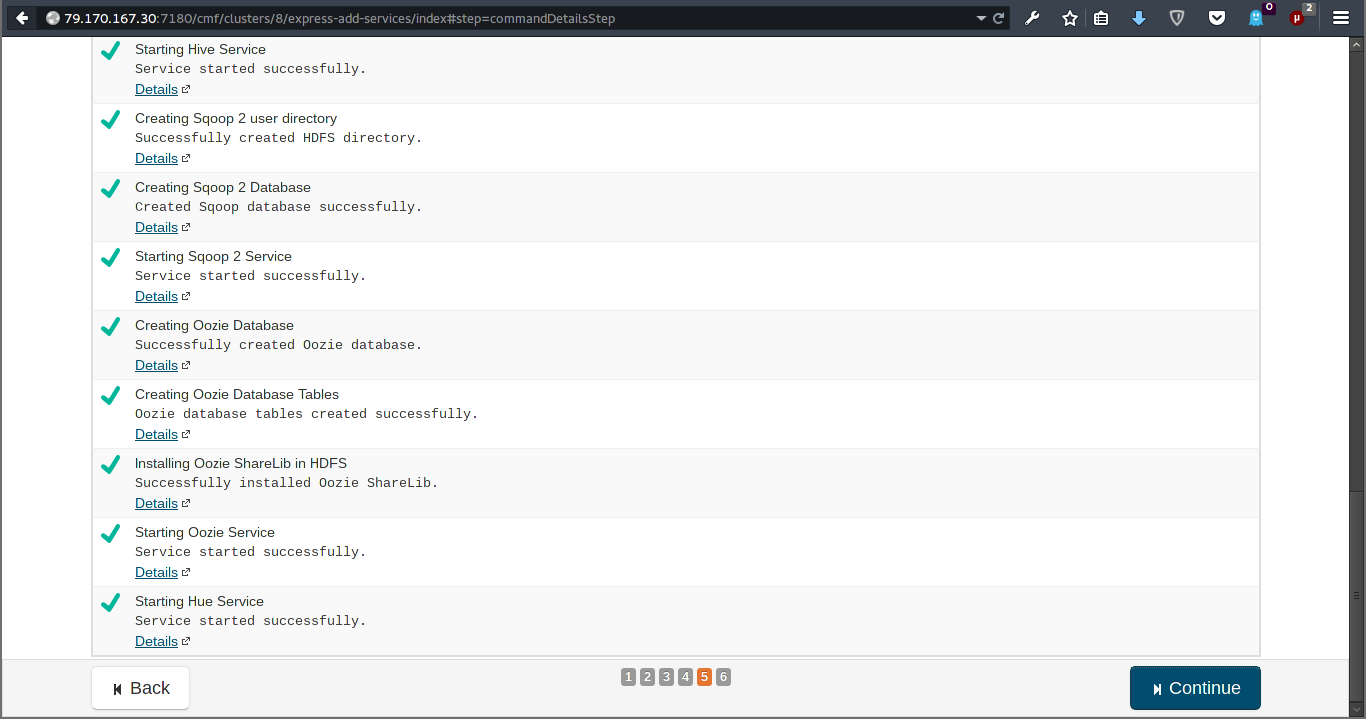
\includegraphics[width=1.0\textwidth]{image-038}
    \caption{Успешная установка компонентов}
\end{figure}

\newpage

\begin{figure}[ht!]
    \center
    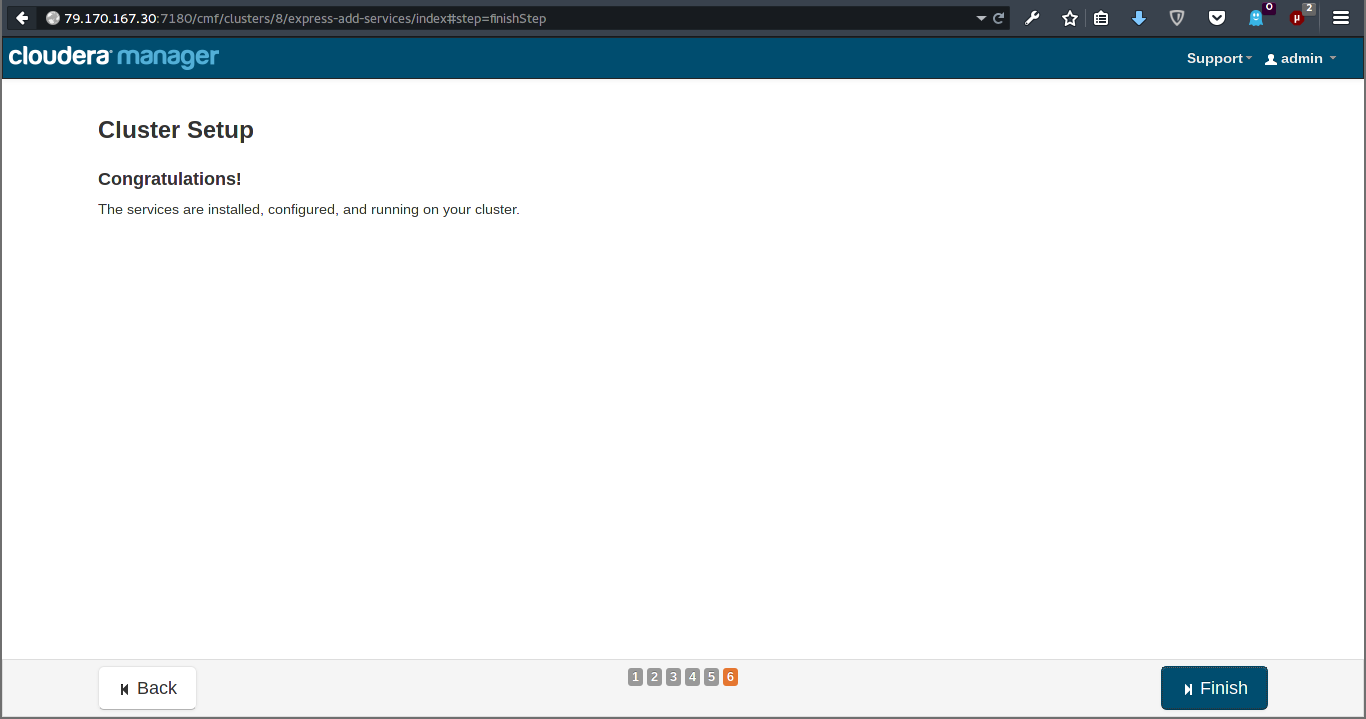
\includegraphics[width=1.0\textwidth]{image-039}
    \caption{Окончание установки компонентов}
    \label{img:last}
\end{figure}

\newpage

\section{Проверка работоспособности}
Для проверки работоспособности сконфигурированного кластера произведём тестовый запуск Hadoop. 
Создадим пользователя, через которого будем производить работу с HDFS и Hadoop, и установим ему пароль.
\begin{lstlisting}
$ sudo useradd -g hduser hduser
$ sudo passwd hduser
\end{lstlisting}
Создадим каталог пользователя в HDFS
\begin{lstlisting}
$ sudo -u hdfs hadoop fs -mkdir /user/hduser/
\end{lstlisting}
Сменим права на данный каталог
\begin{lstlisting}
$ sudo -u hdfs hadoop fs -chown hduser /user/hduser
\end{lstlisting}
Теперь можно использовать данного пользователя для работы с HDFS.
\begin{lstlisting}
$ su hduser
\end{lstlisting}
Создадим каталог для тестовых данных
\begin{lstlisting}
$ hadoop fs -mkdir /user/hduser/input
\end{lstlisting}
Разместим данные в нём
\begin{lstlisting}
$ hadoop fs -put /etc/hadoop/conf/*.xml /user/hduser/input 
\end{lstlisting}
Теперь можно запускать Hadoop на обработку
\begin{lstlisting}
$ hadoop jar /hadoop/cloudera/parcels/CDH/jars/\
   hadoop-mapreduce-examples-2.6.0-cdh5.4.4.jar grep /user/hduser/input /user/hduser/output 'dfs[a-z.]+'
\end{lstlisting}
При успешном завершении в каталоге \emph{/user/hduser/output} появиться следующие файлы
\begin{lstlisting}
Found 2 items
-rw-r--r--   3 hduser supergroup          0 2015-07-26 13:59 /user/hduser/output/_SUCCESS
-rw-r--r--   3 hduser supergroup        390 2015-07-26 13:59 /user/hduser/output/part-r-00000
\end{lstlisting}
Со следующим содержимым
\begin{lstlisting}
$ hadoop fs -cat /user/hduser/output/*
1   dfs.hosts
1   dfs.namenode.acls.enabled
1   dfs.client.domain.socket.data.traffic
1   dfs.client.read.shortcircuit
1   dfs.blocksize
1   dfs.namenode.name.dir
1   dfs.datanode.hdfs
1   dfs.client.read.shortcircuit.skip.checksum
1   dfs.client.use.datanode.hostname
1   dfs.namenode.servicerpc
1   dfs.domain.socket.path
1   dfs.namenode.http
1   dfs.https.address
1   dfs.replication
1   dfs.https.port
1   dfs.groups
\end{lstlisting}
На данном этапе подготовка завершена.

\chapter{Установка дополнительного ПО}
\section{Установка программ из репозитория}
Программы из репозитория CentOS устанавливаются следующей командой
\begin{lstlisting}
$ sudo yum install <program>
\end{lstlisting}

\subsection{Maven}
\begin{lstlisting}
$ sudo wget http://repos.fedorapeople.org/repos/dchen/apache-maven/\
    epel-apache-maven.repo -O /etc/yum.repos.d/epel-apache-maven.repo
$ sudo yum install apache-maven
\end{lstlisting}
При появлении проблем с \emph{Maven} измененить следующий параметр на пустое значение
\begin{lstlisting}
$ export M2_HOME=""
\end{lstlisting} 

\subsection{Lucene}
\begin{lstlisting}
$ sudo yum install lucene
\end{lstlisting}

\subsection{Tomcat}
\begin{lstlisting}
$ sudo yum install tomcat6
\end{lstlisting}
Запуск сервиса производиться любой из представленных команд
\begin{lstlisting}
$ sudo service tomcat6 start
$ sudo /etc/init.d/tomcat6 start
\end{lstlisting}

\subsection{Mr.LDA}
\begin{lstlisting}
$ git clone https://github.com/lintool/Mr.LDA.git
$ mvn clean package
\end{lstlisting}

\section{Сборка Python 3 и установка дополнительных модулей}
Для сборки и установки \emph{Python 3} и \emph{pip} необходимо установить дополнительные программы
\begin{lstlisting}
$ sudo yum groupinstall "Development tools"
$ sudo yum install zlib-devel bzip2-devel openssl-devel ncurses-devel \
    sqlite-devel readline-devel tk-devel gdbm-devel db4-devel libpcap-devel \
    xz-devel
\end{lstlisting}

Переходим непосредственно к сборке и установке\cite{python}
\begin{lstlisting}
$ wget http://www.python.org/ftp/python/3.3.2/Python-3.3.2.tar.bz2 -O /var/tmp/Python-3.3.2.tar.bz2
$ bzip2 -cd /var/tmp/Python-3.3.2.tar.bz2 | tar xvf -
$ cd Python-3.3.2
$ ./configure
$ make -j64
$ sudo make install
$ sudo ln -s /usr/local/bin/python3 /usr/bin/python3
\end{lstlisting}

Установим менеджер пакетов \emph{pip}\cite{pip}
\begin{lstlisting}
$ wget https://bitbucket.org/pypa/setuptools/raw/bootstrap/ez_setup.py
$ sudo /usr/local/bin/python3.2 ez_setup.py
$ sudo /usr/local/bin/easy_install-3.2 pip
\end{lstlisting}

Для использования python с \emph{PostgreSQL} необходимо установить пакет \emph{py-postgresql}
\begin{lstlisting}
$ sudo /usr/local/bin/pip py-postgresql
\end{lstlisting}

\section{Настройка vsftpd}
Установка \emph{vsftpd} (Very Secure FTPD) производится из репозитория
\begin{lstlisting}
$ sudo yum install vsftpd
\end{lstlisting}
Редактируем конфигурационные файлы 
\begin{lstlisting}
$ sudo vim /etc/vsftpd/vsftpd.conf
anonymous_enable=NO
local_enable=YES
write_enable=NO
local_umask=044
anon_upload_enable=NO
anon_mkdir_write_enable=NO
dirmessage_enable=YES
xferlog_std_format=YES
async_abor_enable=YES
ascii_download_enable=YES
chroot_local_user=YES
chroot_list_enable=YES
ls_recurse_enable=YES
listen=YES
hide_ids=YES
anon_root=/hadoop/files
local_root=/hadoop/files
pam_service_name=vsftpd
userlist_enable=YES
userlist_file=/etc/vsftpd/ftpusers
user_config_dir=/etc/vsftpd/users/
tcp_wrappers=YES
guest_enable=YES
\end{lstlisting}

Cоздаём виртуальных пользователей
\begin{lstlisting}
$ sudo vim /etc/pam.d/vsftpd
auth    required        pam_userdb.so   db=/etc/vsftpd/vsftpd_login
account required        pam_userdb.so   db=/etc/vsftpd/vsftpd_login
$ sudo vim /etc/vsftpd/logins.txt
<username-1>
<password-1>
<username-2>
<password-2>
...
\end{lstlisting}

Генерируем БД для виртуальных пользователей
\begin{lstlisting}
$ sudo db_load -T -t hash -f /etc/vsftpd/logins.txt /etc/vsftpd/vsftpd_login.db
$ sudo rm /etc/vsftpd/logins.txt
$ sudo chmod 600 /etc/vsftpd/vsftpd_login.db
\end{lstlisting}

Добавляем в демон в автозапуск и запускаем
\begin{lstlisting}
$ sudo chkconfig vsftpd on
$ sudo service vsftpd start
\end{lstlisting}

Проверку работоспособности демона можно произвести встроенной утилитой \emph{ftp}
\begin{lstlisting}
$ ftp localhost
\end{lstlisting}

\section{Сборка Moses}
\subsection{Сборка необходимых инструментов}
Все действия в основном производятся в каталоге \emph{/hadoop/tmp/}. 
Дальнейшие действия являются адаптацией следующих источников \cite{moses:baseline, moses:dev}.

Добавляем репозиторий в систему и устанавливаем пакет \emph{boost}
\begin{lstlisting}
$ sudo wget http://repo.enetres.net/enetres.repo -O \
  /etc/yum.repos.d/enetres.repo
$ sudo yum install boost-devel
\end{lstlisting}

Клонируем репозиторий \emph{Giza++} и собираем его
\begin{lstlisting}
$ git clone https://github.com/moses-smt/giza-pp.git
$ cd giza-pp
$ make -j64
$ cd /hadoop/tmp
\end{lstlisting}

Клонируем репозиторий \emph{moses}
\begin{lstlisting}
$ git clone https://github.com/moses-smt/mosesdecoder.git
\end{lstlisting}

Делаем файл \emph{bjam} исполняемым и производим сборку
\begin{lstlisting}
$ chmod +x bjam
$ ./bjam -j64
\end{lstlisting}

Создаём папку для \emph{Giza++} в каталоге moses и производим копирование
\begin{lstlisting}
$ mkdir tools
$ cp ../giza-pp/GIZA++-v2/GIZA++ ../giza-pp/GIZA++-v2/snt2cooc.out \
../giza-pp/mkcls-v2/mkcls tools
$ cd /hadoop/tmp
\end{lstlisting}

Загружаем \emph{IRSTLM}, распаковываем и производим сборку
\begin{lstlisting}
$ wget http://downloads.sourceforge.net/project/irstlm/irstlm/irstlm-5.80/irstlm-5.80.08.tgz
$ tar zxvf irstlm-5.80.08.tgz
$ cd irstlm-5.80.08/trunk
$ ./regenerate-makefiles.sh
$ ./configure --prefix=/hadoop/tmp/irstlm
$ make install
\end{lstlisting}

\subsection{Подготовка Corpus для обучения}
Создаём папку для \emph{corpus} и загружаем данные для обучения
\begin{lstlisting}
$ mkdir corpus
$ cd corpus
$ wget http://www.statmt.org/wmt13/training-parallel-nc-v8.tgz
$ tar zxvf training-parallel-nc-v8.tgz
\end{lstlisting}

Перед запуском необходимо убедиться, что для Perl установлен модуль \emph{Time/HiRes.pm}.
При его отсутствии устанавливаем следующей командой
\begin{lstlisting}
$ sudo yum install perl-Time-HiRes
\end{lstlisting}

Производим разбивку данных
\begin{lstlisting}
$ ../mosesdecoder/scripts/tokenizer/tokenizer.perl -l en \
  < ./training/news-commentary-v8.fr-en.en \
  > ./news-commentary-v8.fr-en.tok.en
$ ../mosesdecoder/scripts/tokenizer/tokenizer.perl -l fr \
  < ./training/news-commentary-v8.fr-en.fr \
  > ./news-commentary-v8.fr-en.tok.fr
\end{lstlisting}

Используем обучение с помощью скрипта \emph{train-truecaser}
\begin{lstlisting}
$ ../mosesdecoder/scripts/recaser/train-truecaser.perl \
  --model ./truecase-model.en \
  --corpus ./news-commentary-v8.fr-en.tok.en
$ ../mosesdecoder/scripts/recaser/train-truecaser.perl \
  --model ./truecase-model.fr \
  --corpus ./news-commentary-v8.fr-en.tok.fr
\end{lstlisting}

Используем скрипт \emph{truecase}
\begin{lstlisting}
$ ../mosesdecoder/scripts/recaser/truecase.perl \
  --model ./truecase-model.en \
  < ./news-commentary-v8.fr-en.tok.en \
  > ./news-commentary-v8.fr-en.true.en
$ ../mosesdecoder/scripts/recaser/truecase.perl \
  --model ./truecase-model.fr \
  < ./news-commentary-v8.fr-en.tok.fr \
  > ./news-commentary-v8.fr-en.true.fr
\end{lstlisting}

Производим чистку ограничивая длину предложения 80 символами
\begin{lstlisting}
$ ../mosesdecoder/scripts/training/clean-corpus-n.perl \
  ./news-commentary-v8.fr-en.true fr en \
  ./news-commentary-v8.fr-en.clean 1 80
\end{lstlisting}

\subsection{Обучение модели}
\begin{lstlisting}
$ mkdir /hadoop/tmp/lm
$ cd /hadoop/tmp/lm
$ ../irstlm/bin/add-start-end.sh \
  < ../corpus/news-commentary-v8.fr-en.true.en \
  > news-commentary-v8.fr-en.sb.en
$ export IRSTLM=/hadoop/tmp/irstlm/
$ ../irstlm/bin/build-lm.sh -i news-commentary-v8.fr-en.sb.en \
  -t ./tmp -p -s improved-kneser-ney \
  -o news-commentary-v8.fr-en.lm.en
$ ../irstlm/bin/compile-lm --text=yes \
  news-commentary-v8.fr-en.lm.en.gz news-commentary-v8.fr-en.arpa.en
$ ../mosesdecoder/bin/build_binary \
  news-commentary-v8.fr-en.arpa.en news-commentary-v8.fr-en.blm.en
$ mkdir ../working; cd ../working
$ nohup nice ../mosesdecoder/scripts/training/train-model.perl -root-dir train \
  -corpus ../corpus/news-commentary-v8.fr-en.clean \
  -f fr -e en -alignment grow-diag-final-and -reordering msd-bidirectional-fe \
  -lm 0:3:/hadoop/tmp/lm/news-commentary-v8.fr-en.blm.en:8 \
  -external-bin-dir ../mosesdecoder/tools/ >& training.out &
\end{lstlisting}
Ожидаем завершения обучения модели (может длится очень долго).

\subsection{Запуск moses}
Запускаем \emph{moses} для проверки работоспособности перевода
\begin{lstlisting}
$ ./mosesdecoder/bin/moses -f ./working/train/model/moses.ini
\end{lstlisting}
Необходимо подождать загрузки данных в память, а потом можно вводить текст для перевода в терминале.

\subsection{Сборка с поддержкой xmlrpc-c и irstlm}
Устанавливаем \emph{xmlrpc-c} из репозитория
\begin{lstlisting}
$ sudo yum install xmlrpc-c-devel
\end{lstlisting}

Или скачиваем последнюю версию используя \emph{svn} и производим сборку
\begin{lstlisting}
$ svn checkout http://svn.code.sf.net/p/xmlrpc-c/code/advanced xmlrpc-c
$ cd xmlrpc-c
$ ./configure --prefix=/hadoop/tmp/xmlrpc
$ make install -j64
\end{lstlisting}

Переходим в каталог \emph{/hadoop/tmp/mosesdecoder} и запускаем сборку следующей командой
\begin{lstlisting}
./bjam --with-irstlm=/hadoop/tmp/irstlm/ --with-xmlrpc-c=/hadoop/tmp/xmlrpc -j64
\end{lstlisting}
В случае установки \emph{xmlrpc-c} из репозитория, то можно опустить флаг \emph{with-xmlrpc-c} -- 
\emph{bjam} сам определит, что в системе стоит этот пакет и использует его.

При успешном завершении сборки можно можно запускать \emph{moses} в режиме сервера следующей командой
\begin{lstlisting}
$ ./mosesdecoder/bin/moses-server -f ./working/train/model/moses.ini
\end{lstlisting}

\newpage

\chapter{Заключение}
В результате выполнения можно заключить следующее:
\begin{enumerate}
    \item Проведён анализ технической документации и других материалов по теме работы.
    \item Произведена настройка хост-машин используемых в кластере.
    \item Произведена установка программных компонентов: Cloudera CDH, Tomcat, 
    Lucene, Maven, vsftpd.
    \item Произведена сборка и установка программных компонентов: Python 3, pip, Moses, Mr.LDA.
    \item Произведён перенос патентных данных на жёсткий диск кластера.
    \item Запущен Mr.LDA на обработку патентных данных и получен результат работы.
    \item Произведено подробное описание процесса установки и настройки кластера и 
        дополнительных компонент.
\end{enumerate}

\newpage

\renewcommand{\bibname}{Список использованных источников}
\addcontentsline{toc}{chapter}{Список использованных источников}
\begin{thebibliography}{10}
    \bibitem{parcels} Known Issues Fixed in Cloudera Manager 4.7.2
        [Electronic resource]~--- Available at: 
        \url{http://www.cloudera.com/content/cloudera/en/documentation/cloudera-manager/v4-7-3/Cloudera-Manager-Release-Notes/cmrn_fixed_in_4_7_2.html}
    \bibitem{python} Anderson, S. Install Python 3 on CentOS 6.5 Server
        [Electronic resource]~---~Available at: 
        \url{http://www.shayanderson.com/linux/install-python-3-on-centos-6-server.htm}
    \bibitem{pip} How to Install Python 3.2.2 on CentOS 6.5 amd64 Preserving Its Original 
        Python Installation (2.6.6) [Electronic resource]~---~Available at:
        \url{http://superuser.com/questions/773949/how-to-install-python-3-2-2-on-centos-6-5-amd64-preserving-its-original-python-i}
    \bibitem{moses:baseline} Moses Installation: Baseline [Electronic resource]~---~Available at:
        \url{http://www.statmt.org/moses/?n=Moses.Baseline}
    \bibitem{moses:dev} Getting Started with Moses [Electronic resource]~---~Available at:
        \url{http://www.statmt.org/moses/?n=Development.GetStarted}
\end{thebibliography}